

\documentclass[11pt]{article}

\ExplSyntaxOn % providing \expandableinput
\cs_new:Npn \expandableinput #1
  { \use:c { @@input } { \file_full_name:n {#1} } }
\ExplSyntaxOff

\usepackage{amsmath,amsthm,amssymb, pdfpages,mathtools}
\usepackage{color}
\usepackage{array}
\usepackage{gastex}
\usepackage{subfigure}
\usepackage[normalem]{ulem}
\usepackage{xcolor,psfrag,graphicx}
\usepackage{setspace}
\usepackage{natbib}
\usepackage{lscape}
\usepackage{enumerate}
\usepackage{appendix}
\usepackage[hidelinks, hypertexnames=false]{hyperref}
\usepackage{lscape}
\usepackage{tabularx}
\usepackage{threeparttable}
\usepackage{caption}
\usepackage{booktabs}
\usepackage{longtable}
\usepackage{fullpage}
\usepackage{url}
\usepackage{setspace}
\usepackage{mathpazo}
\usepackage{rotating}
\usepackage{titlesec}
\usepackage{mdwlist}
\usepackage{paralist}
\usepackage{IEEEtrantools}  	% replacing arrays and tables
\usepackage{CJKutf8}  		% display Chinese
\usepackage{epigraph}
\usepackage{environ}
\usepackage{dsfont}
\usepackage{afterpage}
\usepackage[pagewise]{lineno}
\usepackage{xurl}

\usepackage{multirow}					% Create rows in tables that span multiple columns
\usepackage{dcolumn}
\usepackage{tabularx}
\usepackage{float}
\usepackage[T1]{fontenc}
\usepackage{makecell}
\usepackage{rotating}
\usepackage{lscape}



\setcounter{MaxMatrixCols}{10}

\setlength{\evensidemargin}{0.0in}
 \setlength{\oddsidemargin}{0.0in}
 \setlength{\textwidth}{6.5in}
 \topmargin -0.25in
 \textheight 8.5in
 \hfuzz=50pt
 \pagestyle{plain}
\newcommand{\eqthreshn}{{t^*_N}}
\newcommand{\pnd}{1-p+pF(\eqthreshn)}
\newcommand{\ppnd}{\big(1-p+pF(\eqthreshn)\big)}
\newcommand{\eqmfreq}{{\omega^*}}
\newcommand{\eqmfreqn}{{\omega^*_N}}
\newcommand{\eqmfreqnp}{{\omega^*_{N+1}}}
\newcommand{\eqthresh}{{t^*}}
\newcommand{\eqthreshX}{{t^{**}}}
\newcommand{\nbar}{{\overline{N}}}
\newcommand{\wlim}{\omega_\infty}
\newcommand{\wdye}{\hat{\omega}}
\newcommand{\tdye}{\hat{t}}
\newcommand{\limn}{\lim_{N\to\infty}}
\newcommand{\fsn}{\omega_N^*}
\newcommand{\eqprize}{\phi^*}
\newcommand{\moprize}{\phi^M}
\newcommand{\dif}{\;\mathrm{d}}
\newcommand{\diffp}[2]{\frac{\partial #1}{\partial #2}}
\newcommand{\diff}[2]{\frac{\dif #1}{\dif #2}}
\renewcommand{\Re}{\mathbb{R}}                             
\def\endproof{{\quad}$\blacksquare$}
\newcommand{\indicator}[1]{\mathbbm{1}_{\left[ {#1} \right]}}
\newtheorem{theorem}{Theorem}
\newtheorem{proposition}{Proposition}
\newtheorem{prop}{Proposition}
\newtheorem{example}{Example}
\newtheorem{assumption}{Assumption}
\newtheorem{corollary}[theorem]{Corollary}
\newtheorem{acknowledgement}[theorem]{Acknowledgement}
\newtheorem{definition}{Definition}
\newtheorem{lemma}{Lemma}
\newtheorem{remark}{Remark}
\newtheorem{condition}[theorem]{Condition}
 \setlength{\evensidemargin}{0.0in}
 \setlength{\oddsidemargin}{0.0in}
 \setlength{\textwidth}{6.5in}
 \topmargin -0.25in
 \textheight 8.5in
 \hfuzz=50pt
 \pagestyle{plain}
\newcommand{\Change}[1]{{\color{red}#1}}
\renewcommand{\theenumi}{\roman{enumi}}            
\renewcommand{\labelenumi}{(\theenumi)}

%%%%%%%%%%%%%%%
% Page Format %
%%%%%%%%%%%%%%%
 \setlength{\evensidemargin}{0.0in}
 \setlength{\oddsidemargin}{0.0in}
 \setlength{\textwidth}{6.5in}
 \topmargin -0.25in
 \textheight 8.5in
 \hfuzz=50pt
 \pagestyle{plain}





\begin{document}
\title{\textbf{Seeing is Believing: Identity, Inequality, and the Impact of Television on the Hispanic Achievement Gap}%Unravel}
\thanks{Many appreciated suggestions, critiques and encouragement were provided by Leonardo Bursztyn, Lucas Cusimano, Benjamin Enke, Victor Lima, Aakaash Rao, Jaya Wen, David Yang, and Kotaro Yoshida, seminar participants at EPoD, Harvard PE, and the University of Chicago Honors Thesis Workshop as well as Mark Colombo for technical advice on televisions. }\\
}



\author{Andrew Kao\thanks{Harvard University. Email: \texttt{andrewkao@fas.harvard.edu}} }

%\begin{center}
\date{October 2021}
{\vspace{-5ex}}
%\end{center}


\maketitle

\begin{abstract}
\noindent  Can identity reduce inequality? Using a spatial regression discontinuity arising from FCC regulation, I investigate the impact of Spanish Language Television (SLTV) on Hispanic students in public schools. I find that SLTV improves academic performance and helps close the Hispanic achievement gap. I marshal three of sources of evidence that each indicate an identity mechanism is at play: (1) more Hispanic students are labelled `limited English proficiency' and bullied on the basis of their ethnicity in SLTV schools, (2) Hispanic students perform better academically in locales where SLTV programming focuses more on the Hispanic identity, and (3) Hispanics with access to SLTV differentially visit Hispanic branded establishments more frequently. Collectively, they suggest that identity is a mechanism through which SLTV reduces the Hispanic achievement gap.\\\\
\textbf{JEL Codes:} I24, J15, L82, Z13.\\
\textbf{Keywords:} Hispanic, television, education, identity
\end{abstract}




\newsavebox{\tablebox} \newlength{\tableboxwidth}

\setlength{\baselineskip}{22pt}

\renewcommand{\thefootnote}{\fnsymbol{footnote}}


\thispagestyle{empty}

\newpage 
\renewcommand{\thefootnote}{\arabic{footnote}}

\pagebreak 
\setcounter{page}{0}


\onehalfspacing

%\tableofcontents

\newpage

\setcounter{page}{1}
\section{Introduction}

%\begin{quotation}
%\textit{[Television] has altered every phase of the American vision and identity. }
%\begin{flushright} - Marshall McLuhan, \textit{War and Peace in the Global Village}\end{flushright}
%\end{quotation}

The Hispanic achievement gap is wide and persistent. Hispanics face the lowest high school and college completion rates out of all major ethnic and racial groups in the United States.\footnote{ See \cite{tienda_hispanicity_2009}. This achievement gap extends to many more educational outcomes, from test scores to disciplinary incidents to enrolment in advanced classes. Factors such as segregation \citep{cascio_cracks_2012}, XXX, XXX exacerbate the achievement gap, whereas interventions such as providing free computers \citep{fairlie2012academic} XXX help close it.  TODO: other cites on the achievement gap. } In this paper, I argue that Spanish Language Television (SLTV) is a media technology that has reduced educational inequality, and that moreover, these gains in Hispanic student performance can be attributed (at least in part) to a heightened sense of a Hispanic identity.
% TODO: use citations and figures in https://www.colorincolorado.org/article/closing-achievement-gap-focus-latino-students-0
% move footnote into main draft?

Despite the rise of the internet, broadcast Spanish Language TV remains an important fixture of Hispanic households. 78\% of Spanish-dominant households watch SLTV (and 50\% of multi-language Spanish-speaking homes do). In 2010, every single one of the top 10 shows watched by Hispanics were Spanish language programs \citep{pardo_three_2011}. By investigating Spanish Language TV, I take a closer look at Hispanic communities and examine the ties between SLTV, identity, and education. 

To identify the causal effect of SLTV, I follow \cite{velez_tuning_2019} and exploit a spatial regression discontinuity arising from a Federal Communications Commission (FCC) regulation. This regulation grants federal protection of a TV station’s broadcast signal only within a certain distance of a station’s main antenna. Thus, households and schools just inside a TV station's coverage contour should be observably similar to those just outside the contour, except for the presence of broadcast and satellite TV. I argue that this allows me to identify the causal effect of SLTV, given several features: (1) contours are mechanically decided by a formula involving geographical features and antenna strength, (2) contours are large and tend to cut across small towns, rather than dense urban areas which corporations might try to capture for profitability reasons (urban centers fall squarely within contours), (3) SLTV stations were often built before this regulation was imposed, (4) demographic and other controls across the regression discontinuity are similar, and (5) Hispanics do not differentially migrate across contours, minimizing the possibility of selection. To further dispel concerns over potential confounds, I employ a difference-in-discontinuities design, comparing outcomes for Hispanic students against Asian students in schools with and without SLTV based on a 100 kilometer cut-off to SLTV coverage contours.\footnote{I compare against Asian rather than white students because they are much less likely to identify as Hispanic.} 

I verify the relevance of this instrument's first stage by employing the difference-in-discontinuities approach with the American Time Use Dataset. I find that Hispanics watch 10 minutes more of TV when within coverage contours, a plausible lower bound for the amount of extra Spanish Language TV watched if Hispanics substitute watching English programs with Spanish ones. I further show that Hispanics watch more TV with their children---Hispanic students, in other words. Notably, non-Hispanics do not exhibit differential TV viewership across SLTV coverage contours.
	
Next, I utilize the Civil Rights Data Collection to analyze the effect of SLTV on Hispanic students in public schools. Academic outcomes improve across the board: compared to Asians, Hispanics with SLTV are 16\% more likely to take the SAT or ACT, 27\% more likely to enrol in calculus and higher math, and pass 8\% more AP exams. These gains are also present in absolute terms, extend to other academic outcomes, and remain qualitatively similar under a variety of robustness tests, establishing that SLTV reduces the Hispanic achievement gap.

Given this finding, I then marshal three sources of evidence that each indicate an identity mechanism may drive these results. First, using the same data, I show that Hispanic students are differentially classified as having ‘limited English proficiency’ under SLTV despite greater general academic achievement, a likely outcome if these students shift from English to Spanish mastery due to the presence of SLTV. Furthermore, Hispanic students are also differentially bullied more on the basis of their ethnicity, directly indicating a more salient identity that other students may target. Second, I use archive.org’s TV transcript database to classify the proportion of programs in each SLTV station that focus on the Hispanic identity. I show that locales with a greater amount of SLTV programming focused on the Hispanic identity are associated with stronger Hispanic academic performance when compared against locales with fewer such programs on identity. However, a greater amount of programming focused on education \& schools or positive role models for children each have a null effect on Hispanic performance. This indicates that the content of these television programs matter, and that identity is a primary channel through which these gains are attained. Finally, I use foot-traffic data from Safegraph to demonstrate the general strengthening of the Hispanic identity under SLTV. Hispanics with SLTV are differentially more likely to visit Hispanic branded restaurants and recreation establishments. Conducting a placebo exercise, I find that Hispanics with SLTV are no more likely to visit Brazilian, Greek, and Korean establishments. This speaks to the specific strengthening of the Hispanic identity versus a broader Latin American one. Collectively, these results suggest that identity is an important mechanism through which SLTV reduces inequality and the Hispanic achievement gap. 

\paragraph{Literature} Americans spend an average of three hours a day watching TV---more than any other activity bar sleep. Accordingly, a large literature has examined the impact that television has on education. Prior work has frequently been correlational and findings remain conflicted: one line of research contends that TV is as a distraction which `rots' the mind and harms student outcomes \citep{zavodny_does_2006},\footnote{ See \cite{aksoy2000panel}, \cite{hornik1981out}, and \cite{keith1986parental}. This theory enjoys popular support (see \cite{winn_plug-drug_2002} or \cite{gentile_well-child_2004} which finds broad support for the theory among paediatricians). \cite{huang2010dynamic} and \cite{nakamuro2015television} use more sophisticated panel data approaches and also find negative (but smaller) effects.} while another line of inquiry has found consistent null effects.\footnote{ \cite{gaddy1986television}, \cite{gortmaker1990impact}, and \cite{hu2020relationship} take correlational approaches, while \cite{munasib2010idiot} and \cite{kureishi2013does} use self-reportedly weak instruments that may generate the null.} I contribute to this literature by taking a quasi-experimental approach. \cite{gentzkow_preschool_2008} are closest to this paper in using a difference-in-difference strategy to find that TV improves student test scores---particularly among nonwhite students and English language learners. 

Others have studied the effect of television on Hispanic communities. \cite{oberholzer-gee_media_2009} demonstrate that the presence of Spanish language local news increases Hispanic voter turnout, whereas  \cite{velez_tuning_2019} (who develop the instrument used in this paper) find that SLTV depresses voter turnout. \cite{trujillo_devil_2012} run an experiment measuring trust in the government and the census based on a scripted soap opera scene. I extend on this literature by moving beyond the political realm, arguing that the consequences of SLTV are large in educational settings too, and also provide the first evidence on a mechanism through which SLTV operates: identity.

There is a growing literature that looks at how identity can influence behaviour. This has been studied through theory, in the lab, and the field.\footnote{ See \cite{akerlof2000economics}, \cite{benjamin_social_2007}, \cite{benjamin_religious_2010}, and \cite{bursztyn2019moral}, among others.} However, the underlying forces that construct identity (rather than simply triggering them via priming or other short-term interventions) are less well understood. \cite{bisin_bend_2010}, \cite{atkin_how_2019}, and \cite{bazzi_unity_2019} encompass some recent studies on this topic, and all come to the conclusion that intergroup tensions or differences lead to a strengthening of identity. \cite{alesina2013origins} take the long view and show how gender norms can be traced back to early agricultural practices. I contribute to this literature by proposing a media-based channel through which identity may be strengthened and influence action. This is closest to work such as \cite{jensen_power_2009} and \cite{gentzkow_media_2004}, which establish a link between media \& gender norms and media \& anti-Americanism respectively.\footnote{ Other related work on the impact of mass media on social outcomes include \cite{ferrara_soap_2012}, \cite{kearney_media_2015},  \cite{olken_television_2009}, \cite{dellavigna_fox_2007},  \cite{yanagizawa-drott_propaganda_2014}, and \cite{putnam_bowling_2001}. For an overview, see \cite{dellavigna_economic_2015}.} 

Finally, in the education and psychology literature, the stereotype threat phenomenon pinpoints minority identities as a root cause of achievement gaps (\cite{spencer2016stereotype}, \cite{appel2012stereotypes}), leading to the rise of methods such as ``situational disengagement'' \citep{nussbaum2007situational}. This paper suggests that a stronger sense of identity may not have uniformly negative consequences on Hispanic students, creating space for a more positive conception of identity.

% TODO: caveats, include in relevant section
% - Prove the existence of identity mechanism, but does not rule out other mechanisms
% TODO: check caribbean?

% TODO: ICPSR, show that historically they are similar
% TODO: geo-tagged tweets

% some pushback claiming that individual shows can lead to fewer teenage births \citep{kearney_media_2015}


 

% Market sizing: CITE FCC Hispanic TV 
% The Hispanic community is made up of 13.96 million television households nationally, which account for approximately 12.2 percent of the 114.65 million television households in the United States (as of 2012)
% Nationwide, approximately 9.6 percent of U.S. television households are ?broadcast-only;? thus the overwhelming majority subscribe to a pay television service.14 The comparable figure nationwide for Hispanic households is 15.7 percent.15 
% roughly half do not use cable (page 29) - Alternative Distribution Service (ADS)/satellite and broadcast). We find that the majority of Hispanic television households appear to be either cable or Alternative Delivery System (ADS) households. ADS designations refer to households with one or more televisionsetsthatreceiveprogrammingfromoneoffourtypesofsystems: DBS;satellitedish (C-Band); satellite antenna television (SMATV); and multi-channel, multi-point distribution systems (MMDS). Broadcast television households,
% programming split fairly evenly between locally produced segments, news, telenovelas, and paid programming, the latter three of which may come from abroad

% viewed by half of all Spanish-dominant Latinos (http://www.horowitzresearch.com/press/spanish-language-tv-content-remains-integral-to-u-s-hispanics-tv-diet-new-horowitz-survey-shows/)
% better: Nielsen, 78% Spanish-dominant watch Spanish TV, 50% in multi-language homes, over 85% broadcast -- in 2010, top 10 broadcast shows in Hispanic demographic were all Spanish language
% market size: millions in LA, New York etc. https://www.statista.com/statistics/189824/largest-hispanic-television-markets-in-the-united-states-2011/

% broadcast/satellite TV vs cable: https://www.quora.com/What-is-the-difference-between-cable-and-broadcast

% in recent years, highest viewed: Pequeños Gigantes (talent show, kids), El Señor de los Cielos (telenovella, cartel leader),   https://www.statista.com/statistics/497739/spanish-tv-programs-usa/



%% Do everything with d^2
%% spatial errors: http://www.trfetzer.com/using-r-to-estimate-spatial-hac-errors-per-conley/


\paragraph{Layout.} Following this Introduction, Section \ref{s:data} presents the data sources used. Section \ref{s:rd} describes the difference-in-discontinuities empirical strategy and establishes the first stage. Section \ref{s:school} presents evidence that SLTV closes the Hispanic achievement gap. Section \ref{s:mech} presents evidence that an identity mechanism underlies these results. Finally, Section \ref{s:conclusion} concludes with a discussion of research questions opened by the preceding analysis.



\section{Data}\label{s:data}


%\subsection{Broadcast TV and Geography}

\paragraph{Coverage contours}  The central instrument in this paper is the discontinuity in SLTV coverage across coverage contours introduced by FCC regulation. To build the coverage contours of SLTV stations in the United States, I collect a list of the callsigns for all SLTV stations from TMS Media, a large provider of data on TV, movies, and other media.\footnote{ A TV station is defined to be SLTV if at least one of the primary broadcasts languages are Spanish.} There are 103 of these stations located across the United States. These callsigns are matched against data from the FCC's OET Bulletin No.~69 and the FCC's Consolidated DataBase System (CDBS) to directly obtain the coverage contour boundaries in 2015.\footnote{ 2015 coverage contour data is used due to the 'FCC Spectrum Repack' that began in 2018 which altered the reception and coverage for a substantial number of stations. Coverage contours prior to 2015 were generally stable. }  % repack cite: \citep{fletcher_fcc_2018}
Figure~\ref{f:contour_example} presents an example of a coverage contour, while Figure~\ref{f:contours_schools} displays a map of all SLTV contours in the United States.

\paragraph{Time use data} I collect time use data from the American Time Use Survey between 2003-2015 and construct the total amount of time individuals spent watching TV, time spent watching TV with children and parents, time spent on children's education, and demographic variables. Individuals in the data are located at the county level---I classify a given county as falling within a SLTV contour coverage if at least 50\% of its area does. 68,373 individuals in the sample live within 100 kilometers of the contour boundary. Table~\ref{t:summary}, Panel A presents summary statistics for this data.  
	

\paragraph{Public school data} I collect data on public schools from the US Department of Education's Civil Rights Data Collection (CRDC) dataset in 2015. For anti-discrimination and transparency purposes, all public schools in the United States are required to report data to the CRDC on an annualized basis. This data contains information on various indicators of educational performance by demographic category, including SAT/ACT tests taken, calculus courses taken, AP tests passed, students classified under `Limited English Proficiency', students bullied on the basis of ethnicity or race, the number of teachers and students in the school, and more.\footnote{ Comprehensive variable descriptions are provided under \ref{a:auxiliarydata}.} School addresses are geocoded using ArcGIS and coded as receiving SLTV if they fall within a coverage contour. 83,004 schools across 11,065 school districts fall within 100 kilometers of the contour boundary. Figure \ref{f:contours_schools} presents a map of these schools and Table~\ref{t:summary}, Panel B presents summary statistics for this data. 


\paragraph{Television transcript data} To code the content of programs broadcasted by SLTV stations, I make use of archive.org's television transcript database covering the years 2005-2015. Because transcript data is available at the television network level, I assign all affiliate stations data from their parent network.\footnote{ There are nine major Spanish Language TV networks present in the data: Telemundo, Univision, UniMás, Azteca América, PBS, Estrella TV, MundoMax, Enlace TBN, and Mega TV. } For each network in the database, I code the fraction of television programs whose transcripts contain kesywords related to the mechanisms that I study: identity, education, and role models.\footnote{ More sophisticated text analysis techniques such as NLP are not possible due to copyright law restricting direct access to the text corpus. Thus, only keyword searches are feasible. The specific set of keywords used are displayed in Appendix Table~\ref{t:transcript_keywords} and the process for constructing this set is described under \ref{a:auxiliarydata}.}  Table~\ref{t:summary}, Panel C presents summary statistics for this data. 
% TODO: correct time period
% TODO: drop Brazil, Suriname

\paragraph{Foot-traffic data} I gather Safegraph foot-traffic data from 2019 to analyze whether Hispanics differentially visit Hispanic-branded establishments under the presence of SLTV. Safegraph uses location tracking data from mobile phones to compile comprehensive foot-traffic data to over 10 million points of interest around the world. I restrict the analysis to two commercial sectors where ethnic branding is common: food services (NAICS code 72) and arts, entertainment, and recreation (NAICS code 71). Restaurants and other food service establishments are tagged by Safegraph with the type of cuisine served, which I use to classify an establishment as Hispanic or not. Recreation establishments are not tagged, so I match establishment names with the same identity keywords used to classify the transcript data to code establishments as Hispanic. I repeat this for a number of placebo ethnicities: Greek, Korean, and Brazilian. Safegraph provides data on the number of visitors to each establishment at the census block group level. Thus, I use census data and the instrument to impute the number of Hispanics and non-Hispanics, with and without SLTV, who visit each establishment within 100 kilometers of a SLTV coverage contour.\footnote{ Given the potential selection concern of users whose data are covered by Safegraph, I also apply a Heckman correction based on sample moments from the Safegraph data to match the census data to correct the number of visitors in each category.} There are 273,216 establishments included in my sample. Table~\ref{t:summary}, Panel D presents summary statistics for this data. 

\paragraph{Other data} \ref{a:auxiliarydata} describes other data used in the paper. Briefly, they are IPUMS migration data at the origin county-destination county level from 2010-2015, used to test for selection via migration, and the American Community Survey data for county level demographic controls. The appendix also describes in greater detail the data construction process for the datasets above.



\section{Empirical strategy}\label{s:rd}

To isolate the causal effect of Spanish language television, I adapt the technique used in \cite{velez_tuning_2019}  and extend it from two counties to the entirety of the United States. Velez and Newman construct a spatial regression discontinuity based on a FCC (Federal Communications Commission) regulation which determines the distance from a TV station in which the station's broadcast signal is protected from interference.

Digital and satellite TV stations operate by broadcasting signals from a central antenna, and the antenna's field strength at any given point is a mechanical product of several factors: the antenna's ERP (Effective Radiated Power, which is the amount of input power given to the antenna adjusted for antenna idiosyncrasies that may boost or attenuate its effective power), the antenna's HAAT (High Above Average Terrain), and the distance from the point to the antenna. This signal declines in strength with the square of distance, making it subject to interference and general loss of signal. When one gets far enough away from a TV station, this interference becomes widespread and meaningfully impedes TV viewership: the FCC completely repacked the spectrum between 2018-2020 to more efficiently allocate the frequencies on this spectrum and prevent interference.\footnote{ Interference is most common from other TV broadcasters, as even weak signals and signals from adjacent channels (both digital and analog) can cause major reception issues. Distance also aggravates common TV signal quality issues such as ghosting (the appearance of double images due to geographical obstacles/multiple signals) and exacerbates interference from other signals, including radio transmitters (whether commercial, CB, or amateur), and can even result in electrical sources (such as power lines or large motors) disrupting reception.} To safeguard TV signals, the FCC passed in 1997 a series of regulations to protect signals for commercial TV stations from interference. These took the form of contour areas for which service holds at 50\% of locations 10\% of the time, termed a noise-limited bounding contour, inside of which sufficiently strong interfering signals are banned.\footnote{ The relevant sections of federal law are 47 C.F.R. 73.622, 73.623, and 74.704. The FCC's OET Bulletin No. 69 most clearly summarizes and provides guidance on the salient features in this law. These contour interference protection lines are constructed following the Longley-Rice methodology adopted in 1997 and are termed $F(50,10)$ lines. In practice, this regulation is most frequently used to restrict new TV station allotments. There are also $F(50,90)$ lines which demarcate minimum field strength for digital TV service; these coverage contours are strict subsets of the interference contours and are not as suitable for a regression discontinuity as it is likely that people just outside of these contours are still able to access a television signal.} The blue contour line in Figure~\ref{f:contour_example} presents an example of one such coverage contour.
%@CITE https://www.fcc.gov/media/radio/fm-and-tv-propagation-curves
%@CITE White Paper TAC

% interference: https://www.ic.gc.ca/eic/site/smt-gst.nsf/eng/sf01382.html
% law: https://www.ecfr.gov/current/title-47/chapter-I/subchapter-C/part-73/subpart-E/section-73.622

This regulation creates a natural spatial regression discontinuity. Combined with the decaying strength of a TV signal due to distance, this cut-off in broadcast protection creates a split among households and schools just inside and outside of these coverage contours that should be ex ante comparable save for their access to broadcast TV. This is operationalized as a 100 kilometer cut-off from the coverage contour border in my baseline specifications. By studying Spanish Language TV in particular, I should be able to examine its causal effect on Hispanic communities, so long as the location of these contours are uncorrelated with any of the other determinants for the outcomes studied. 

Given that these contours are purely determined by an algorithm and only dependent on physical variables like local elevation and antenna strength, these precise regulatory boundaries are located in more or less random locations. Coverage contours are large enough that they tend to cut across small towns rather than large cities---television networks have not constructed their antennae to be just large enough to only cover the most dense and populous areas.\footnote{ These urban centers fall squarely within the aforementioned $F(50,90)$ lines where minimum field strength must be guaranteed. This implies that network executives aiming to maximize profit, ratings, or audiences, should not have the $F(50,10)$ interference lines used in this paper at the forefront of their decision calculus.} 

Another reassurance is that the interference protection regulation and the Longley-Rice methodology used to determine TV service coverage were only adopted in 1997, making it unlikely that stations were built or adapted in response to the policy. Univision, the largest owner of SLTV stations, was founded in 1955, and had built the vast majority of their television stations and antennas by 1997. Telemundo, the second largest owner of SLTV, was founded in 1984 and the stations it initially acquired were built in 1954. Like most SLTV networks, it primarily expanded through the acquisition of existing stations, rather than building out its own new ones. Nonetheless, one may still believe that SLTV stations target areas with more Hispanic people, or wealthier communities, or more populous areas, all of which are factors that could affect the areas of interest. Hence, I include explicit controls for these variables in regressions.
% @TODO CITE univisino, telemundo


Finally, one may still be worried that unobserved variation across coverage contours could drive the observed results. Therefore, I follow a recent literature on difference-in-discontinuities (\cite{casas2015women}, \cite{grembi2016fiscal}) and employ a design that, in addition to the regression discontinuity, also compares outcomes for Hispanic students against Asian students.\footnote{ I compare against Asian rather than white students because they are much less likely to identify as Hispanic. The achievement gap between Hispanics and Asians tend to be as large, if not larger, than the Hispanic-white achievement gap, making this a result of independent interest.} Thus, any alternative explanation for these results would need to differentially affect Hispanics across these coverage contours.

The instrument therefore consists of two variables interacted: first, an indicator for whether the observation falls within any SLTV station's coverage contour boundary, and second, a Hispanic indicator. To ensure similarity between obervations inside and outside the boundaries, only observations located within a distance of 100 KM of the boundary are kept. The main specification is: %\footnote{ Using a round number in kilometers rather than miles makes this cutoff less likely to be correlated with real-world phenomena in the US.} 

\[ y_{i,j} =  \beta \mathbb{I}[InsideContour_{i,j}] \times \mathbb{I}[Hispanic_{i,j}] + \gamma_k + \delta  X_i + \epsilon_{i,j} \]

where $y_{i,j}$ is an outcome for observation $i$ (which may be an individual, school, or establishment) under demographic category $j \in \{$Hispanic, not Hispanic$\}$, $\gamma_k$ is a school district fixed effect (included when relevant), and $X$ is a vector of controls for the observation. The main coefficient of interest is $\beta$, and in particular, the interaction term between the Inside Contour and Hispanic indicators. 


Two potential concerns remain:
\begin{itemize}
\item \textit{Can we guarantee that it is Hispanic people who watch SLTV?} If it were the case that non-Hispanic people were frequent viewers of SLTV, the main effects could also be attributed to non-Hispanics directly changing their behavior based on SLTV viewership. This could be the case if, for instance, white people treated Hispanics and Asians differently after having viewed SLTV, or Asian students performed worse in schools after watching SLTV. However,  $<1\%$ ofs TV programming watched by non-Hispanics is in Spanish, making such stories unlikely to hold water \citep{noauthor_hispanic_2016}.
% However, only 4\% of total SLTV station programming watched can be attributed to non-Hispanic people, a number that is only as high as it is because some SLTV stations also broadcast in English  (FCC). Similarly,

\item \textit{How do we account for potential selection?} It is theoretically possible that Hispanic people move in response to these television coverage contour boundaries, and that the effects seen are therefore a result of Hispanics self-sorting. If true, this would be a remarkable result---people moving in large numbers for the sake of access to better television. However, using census migration data, I find that Hispanics do not differentially move into or out of counties with access to SLTV. Appendix Tables \ref{t:mig_orig} and \ref{t:mig_dest} present these regression results and suggest that, if anything, Hispanics are \textit{averse} to moving across coverage contour boundaries.



\end{itemize}




\subsection{Evidence of a first stage: do Hispanics in SLTV coverage contours watch more television?}

Over 85\% of Hispanic households own a television. A further 85\% of SLTV viewership occurs over satellite or broadcast television---important because coverage contours are only applicable for these types of television.\footnote{ See \cite{noauthor_hispanic_2016} and \cite{de_la_merced_att_2014}. This fraction of broadcast TV viewership is substantially larger than the national average, 24\%.} Thus, a substantial fraction of Hispanics may be affected by the presence of these coverage contours.
%  Of these, over half get their television content via satellite or broadcast television---

I test for the amount of television watched across these contour boundaries with the American Time Use Survey data. Figure~\ref{f:atus} graphs the minutes of television watched against the distance to the contour boundary: it is clear that Hispanic television viewership increases inside the boundary while non-Hispanic viewership remains flat. However, there is not a sharp break in Hispanic viewership at the border, but rather a continuous increase as one draws closer to the main station---this indicates a fuzzy regression discontinuity, combining the natural effect of distance to the signal with the effect of the FCC interference protection. 

Table~\ref{t:atus_main}, Panel A presents a regression following the main specification. Hispanics watch an average of 10 minutes more television when within the contour, whereas the effect of the contour on non-Hispanics is insignificant. Panel B examines the effect of the contour on minutes of TV watched with one's children: this too increases for Hispanics by 3.5 minutes while not affecting viewership for non-Hispanics. Thus, Hispanics overall and Hispanic students (the children of individuals surveyed) both appear to watch more TV within the coverage contour. But does more TV viewership mean that \textit{Spanish Language} TV viewership increases? Unfortunately, I cannot directly observe the amount of SLTV watched. However, if one reasonably assumes that English and Spanish Language TV are substitutes,\footnote{ Though no direct economic research exists on the substitutability of English and Spanish Language TV, the Department of Justice's ruling on the Univision-HBC merger (68 Fed. Reg. at 66,857 (2003)) interprets these English vs. Spanish language networks as substitutable products.} then these estimates would serve as a lower bound for the increase in SLTV watched by Hispanics. 

% Second, Hispanics consume substantial amounts of television---out of the 115 million households with television in the United States, there are 14 million Hispanic ones, proportional to the overall fraction of households. 

Compared to other viewers of television, Hispanics are also uniquely likely to watch television in a social context rather than watching alone---this is partially driven by the fact that non-Hispanic households have 40\% more TV sets per person than Hispanic ones \citep{coghill_tuning_2018}. This social aspect, wherein SLTV is watched with family and friends, may be one way in which identity is reinforced through television. Appendix Table~\ref{t:atus_foreign}, Panel A shows that Hispanics differentially watch more TV with their parents when inside SLTV coverage contours. Appendix Table~\ref{t:atus_foreign}, Panel B replicates the analysis in Table~\ref{t:atus_main}, Panel A, restricting the sample to only foreign-born residents. These people are less likely to have English mastery and may thus view more foreign-language TV. Accordingly, the panel reports even greater differential TV viewership among foreign-born Hispanics.


% https://www.effectv.com/blog/tuning-hispanic-audiences
% even the largest markets do not locally source more than 20\% of their Spanish language programming - from foreign countries or domestic


%%%%%%%%%% PUBLIC SCHOOLS %%%%%%%%
\section{The impact of Spanish language television on Hispanic educational performance}\label{s:school}

How big is the Hispanic achievement gap in public schools? Table~\ref{t:edu_magnitude}, columns 1 and 3 present the achievement gap between Asians and Hispanics and whites and Hispanics respectively. In almost every outcome of interest, Hispanics trail substantially behind their Asian and white peers. Compared to Asian students, Hispanic students take the SAT or ACT 46.8\% less frequently, take calculus 53.6\% less frequently, and pass 72.3\% less AP examinations. These are startlingly large figures, making it imperative for us to find solutions that can help close the achievement gap.

To determine the effect of SLTV on the Hispanic achievement gap, I apply the main difference-in-discontinuity specification at the school-ethnicity level and compare differential outcomes between Hispanics and Asians while varying the presence of SLTV. I apply the inverse hyperbolic sine transform to all outcome variables in order to study the elasticity, or percentage difference, of these academic outcomes with respect to SLTV. Only schools within 100 KM of the coverage contour boundary are kept and standard errors are clustered at the school district level. 
 
Table~\ref{t:edu_main}, Panel A presents results on the IHS transformed number of SAT and ACT tests taken, Panel B presents results on the IHS transformed number of calculus courses taken, and Panel C presents results on the IHS transformed number of AP exams passed.\footnote{ The sample size changes across panels due to schools not reporting data when it is irrelevant. Not all schools offer the SAT/ACT test or calculus or AP exams. In order for missing data to bias results, selection would need to be correlated with the presence of coverage contours. It is unclear that schools have such an incentive to differentially manipulate reporting along this dimension.} All columns control for school district fixed effects and the number of Hispanic and Asian students in the school. Columns 2 and 3 add controls for the total number of students and teachers in the school, and column 3 adds controls for the school type (elementary, middle, and high school indicators). Results are statistically and economically significant. SLTV differentially improves the number of Hispanics taking the SAT or ACT by 16\% (Panel A), the number of Hispanics taking calculus by 27\% (Panel B), and the number of Hispanics passing an AP exam by 10\% (Panel C). The degree to which this decreases the achievement gap is presented in Appendix Table~\ref{t:edu_magnitude}. 

One may naturally wonder whether Hispanic students only gain in relative terms to their peers. Appendix Table~\ref{t:edu_abs} presents results utilizing only the regression discontinuity instead of the difference-in-discontinuities specification.\footnote{ Due to the high degree of collinearity between school districts and the presence of SLTV, the school district fixed effects must be dropped from this specification.}  Although the estimated coefficients are generally smaller, the effect of SLTV remains positive, indicating that Hispanic students gain in absolute as well as relative terms. These gains in academic performance are present in a variety of other academic outcomes: Appendix Table~\ref{t:edu_extra_achieve} shows that the Hispanic achievement gap is reduced in the number of gifted students (Panel A), advanced math courses taken (Panel B), biology courses taken (Panel C), physics courses taken (Panel D), and chemistry courses taken (Panel E). Appendix Table~\ref{t:edu_magnitude} presents the size of the achievement gap and the degree to which SLTV ameliorates it for these auxiliary outcomes.


\paragraph{Robustness and ruling out alternative hypothesis}

The difference-in-discontinuities strategy should take care of most concerns regarding identification. I next perform several robustness checks and rule out potential alternative hypotheses that may explain the data in Appendix Table~\ref{t:edu_robust}. For each of these checks, I replicate results for SAT and ACT tests as Panels X.X.1, calculus classes taken as Panels X.X.2, and AP exams passed as Panels X.X.3. Baseline results are presented in Panel A.1.

One may be concerned that schools near the outer bounds of the 100 kilometer cutoff may look quite different from one another. I narrow the sample distance cutoff to the contour boundary from 100 kilometers to 50 kilometers and 33 kilometers and find that coefficients remain stable (see Panels A.2 and A.3). One may also be concerned about treatment effects very close to the coverage contour: students who attend a school 1 kilometer outside the contour may in fact live inside the contour, and the interference protection regulation may not be tightly enforced down to the last square foot. Thus, I keep only schools between 25 and 100 kilometers of the contour boundary and find qualitatively similar results (see Panel A.4). Given that television signals decrease with the square of distance from the main station, I additionally add controls for distance and distance$^2$ and find that results are robust (see Panel A.5). Any variation along state or county levels that may ex ante affect school similarity are also absorbed by the school district fixed effects. 

Given the interest in the Hispanic achievement gap and the presence of 0s in the data, it is natural to use the IHS transform on outcome variables. The results are also robust to using the $log(x+1)$ transform instead (see Panel B.1). If one is interested in the numerical difference (rather than percentage change) that SLTV induces, Panel B.2 presents results for raw counts and Panel B.3 presents results for the standardized count of the variables. In each case, results remain positive and significant. Similarly, though results are run at the school level, one may be interested in student-level outcomes. Panel C.1 weights observations by the size of schools whereas Panel C.2 weights observations by the number of students in the given demographic category to make the data representative at the student level; results remain largely unchanged.

The presence of bilingual stations that broadcast in both English and Spanish may alter the interpretation of results if change in Hispanic behavior is driven by these particular stations. There are 14 such stations in the data. Panel D.1 drops these stations and finds that coefficients remain stable. 

Reverse causality could be a concern if TV executives strategically place TV stations to capture certain markets by the edges of the coverage contours. Panel E.1 controls for the station-level determinants of a TV signal's field strength (its antenna's effective radiated power, height above average terrain, radiation center above mean sea level, and presence of a directional antenna), which should account for the factors that a network could manipulate to increase or decrease coverage, and finds that results are robust.\footnote{In practice, the local topography is also important for determining field strength. But if the mountain will not come to Muhammad, then Muhammad must go to the mountain. Thus, controlling for the above technical factors should be sufficient until terraforming is prevalent.} Panel E.2 drops the 11 SLTV stations that were built after 1997 (when the FCC regulation was passed), which may have been constructed with the interference coverage contour in mind; results remain qualitatively similar.

Selection \textit{within} schools may also be a concern: perhaps the worst Hispanic students drop out more under the presence of SLTV, or the best Hispanic students move to private schools in areas without SLTV. I test for this in Appendix Table~\ref{t:edu_retain} and find an insignificant difference in the number of Hispanic students retained across the SLTV boundary.

The main results also remain significant under different treatments of standard errors. Appendix Table~\ref{t:edu_robust}, Panels F.1 and F.2 correct for spatial autocorrelation, accounting for arbitrary spatial clusters and allowing for linear decay in the correlation structure (using the Bartlett kernel). Panel F.3 two-way clusters standard errors by school district and the parent TV network of the closest station. Panel F.4 clusters standard errors at the TV station level. Panel F.5 uses heteroskedasticity robust standard errors.

Finally, one might wonder how SLTV affects the white-Hispanic achievement gap. Panel G.1 presents results using white students as the omitted category instead of Asian students. Hispanics make up even more ground under this specification.

% TODO: table notes for longtable

Taken as a whole, these results suggest that SLTV is a meaningful force that can improve Hispanic student performance in public schools and reduce the achievement gap. Nonetheless, several caveats must be made: first, although taking the SAT and ACT exams, taking higher math, and passing AP exams are all correlated with enrolment in college and higher earnings, I do not actually observe long-run outcomes for these Hispanic students. Thus, it may be the case that SLTV helps the youth but not adults.\footnote{ Though it is in principle possible to employ this difference-in-discontinuity design to these long-run outcomes, I focus on immediate schooling outcomes in this paper and leave the long-run effect as space for potential future work.} Second, although students outcomes in schools improve, this analysis does not speak to a variety of other negative consequences thought to be caused by TV, such as obesity or violence. Finally, these findings are focused on measuring the effect of \textit{Spanish Language} TV, rather than on TV as a whole. It is worth bearing in mind that the literature typically finds null to negative effects of TV, which may lead the positive effects of SLTV to come as a shock to some. Academic brilliancy is not typically associated with the banal, mindless enjoyment of lazing on a couch before a flatscreen. So what might drive these results?



\section{The identity mechanism}\label{s:mech}

In this section, I present evidence to show that a strengthened Hispanic identity is a mechanism through which SLTV improves academic performance. 

Compared to English broadcasts, SLTV is more likely to contain content that is directly salient to a Hispanic person's identity. This is not only because of the language of the broadcast, but also its content: roughly 20\% of programming on SLTVs are telenovelas produced in Latin American countries, with a similar proportion of programming dedicated to non-locally produced news and paid programming.\footnote{ For more information, see \cite{noauthor_hispanic_2016}. } These programs can serve as a direct tie to a viewer's country of origin, supplementing and strengthening their sense of self. % TODO: find footnote cite; if none just use econ TV identity above


\subsection{Identity within schools}

I return to the CRDC public school data used in Section~\ref{s:school} and identify two variables that speak to the strength of one's Hispanic identity: (1) classification as a `Limited English Proficient' (LEP) student, and (2) harassment or bullying on the basis of race, color, or national origin. Table~\ref{t:edu_mech} follows the difference-in-discontinuities specification used in Table~\ref{t:edu_main} and examines the differential effect of SLTV on these outcomes.

Table~\ref{t:edu_mech}, Panel A shows that Hispanics with access to SLTV are 30\% more likely to be classified as a  `Limited English Proficient' (LEP) student when compared to their peers. This decrease in educational performance stands in contrast to all other academic outcomes studied thus far, suggesting that it is not a difference in general intelligence or work ethic that drives this result, but rather an idiosyncratic decline in English speaking ability. Though I do not directly observe the extent to which students speak Spanish, the most parsimonious explanation for this finding is that watching SLTV causes students to attain greater mastery of Spanish, at the cost of their English skills.\footnote{ This decline in English ability is a genuine cost that should be evaluated against the gains made in other academic areas. A full cost-benefit analysis is beyond the scope of this paper.} To guard against the concern that this effect is driven by a purely \textit{perceptual} change of Hispanic students by teachers and administrators, Appendix Table~\ref{t:edu_mech_placebo} shows that the number of Hispanic students classified as disabled under IDEA (Individuals with Disabilities Education Act) does not differentially change with access to SLTV. This panel also serves as a general sanity check, as SLTV should not cause students to develop disabilities. 

Table~\ref{t:edu_mech}, Panel B shows that Hispanics with access to SLTV are also differentially likely to be harassed or bullied on the basis of their ethnicity. Hispanic students with SLTV are more likely to be bullied because they are Hispanic. On the other hand, Appendix Table~\ref{t:edu_mech_placebo} shows that the number of Hispanic students bullied on the basis of their sex does not differentially change across the SLTV contour when compared to their peers. Any mechanism through which SLTV increases the propensity for Hispanic students to be bullied (such as students picking on strong academic performers) would need to reconcile the null result for bullying on sex. My preferred explanation for this finding is that Hispanics watching SLTV make their ethnic identity more salient, making them a greater target for bullying along this particular dimension. This is corroborated by a substantial literature that has shown that increased visibility of (non-majority) ethnicities is associated with them being bullied more.\footnote{ See \cite{scherr_bullying_2009} for a review of this literature.} Appendix Table~\ref{t:edu_mech_abs} shows that LEP classification and bullying based on ethnicity for Hispanics with SLTV also increase in absolute terms. 

Thus, though it is impossible to rule out all other stories that may drive this set of results, there are not many which can explain the reversal in academic ability for only English proficiency and the increased bullying on the basis of ethnicity but not sex among Hispanic students. A strengthened Hispanic identity through SLTV neatly takes care of these considerations.


\subsection{The content of TV programs: narrowing down the mechanisms at play} \label{s:transcripts}

I next turn to the content of these SLTV programs in order to assess three potential mechanisms through which SLTV increases educational performance: (1) SLTV programs strengthening the Hispanic identity, (2) SLTV programs stressing the importance of education, and (3) SLTV programs provide good role models for students. I infer the content of SLTV programs using keyword matching of terms related to each mechanism in the archive.org TV transcript database. To evaluate the strength of each mechanism, I modify the main specification by interacting the difference-in-discontinuity with the salience of each mechanism:

\[ y_{i,j} =  \beta \mathbb{I}[InsideContour_{i,j}] \times \mathbb{I}[Hispanic_{i,j}] \times Mechanism_{s} + \gamma_k + \delta  X_i + \epsilon_{i,j}\] 

where $s$ indexes a given SLTV station, and $Mechanism_s$ is the percentage of programs from the station focused on a given mechanism. The triple interaction term between Inside Contour, Hispanic, and Mechanism yields the elasticity of the outcome with respect to the mechanism, and is thus the coefficient of interest.

Table~\ref{t:transcript_main} displays results for regressions following this specification. I focus first on column 1, measuring the strength of the identity mechanism. The triple interaction term is positive for the outcomes SATs and ACTs taken (Panel A), calculus courses taken (Panel B), and AP exams passed (Panel C). Panels A and B both show strong and significant effects, whereas Panel C is borderline insignificant---it suffers most from power issues due to the low number of schools reporting this data and the demands of a triple difference. These results indicate that SLTV stations increase Hispanic academic performance more when they focus more on the Hispanic identity. Appendix Table~\ref{t:transcript_abs}, column 1, shows the effect of the regression discontinuity interacted with the percentage of programs on identity (comparing only within Hispanic students, and not against Asian students as well), and finds that results remain largely similar. Thus, if these identity-focused shows impart a stronger sense of identity for Hispanics, then this would suggest that identity can be mobilized to close the Hispanic achievement gap.

Turning to Table~\ref{t:transcript_main}, column 2, this suggests that a greater emphasis on education in SLTV programs do not necessarily translate into stronger academic performance among Hispanics when compared to their peers. Although signs are positive for calculus taken (Panel B) and AP exams passed (Panel C), they are insignificant, and the sign on SATs and ACTs taken is negative.\footnote{ This is potentially due to the fact that I cannot measure the valence with which education is treated by SLTV stations. One show may laud the merits of school, while another might paint it as a bore; both would appear in my data as a program focused on education.} Appendix Table~\ref{t:transcript_abs}, column 2, shows a similar effect when looking at Hispanics alone. Returning to the time use data, Appendix Table~\ref{t:atus_edu} shows that parents do not spend any more time with their child on educational activities when they have access to SLTV. Taken together, these findings suggest that SLTV does not improve academic performance by raising the importance of education itself.

Table~\ref{t:transcript_main}, column 3, looks at the percentage of programs that contain good role models for students and children. As in the preceding case of education, the sign on the triple interaction term is mixed and never significant. Appendix Table~\ref{t:transcript_abs}, column 3 shows the interaction between the regression discontinuity and percentage of programs that contain good role models; again, no result is indicative of this mechanism improving student outcomes. It is worth noting that this does not mean that role models have no role to play---it may simply be that their presence in programs that not explicitly targeted at students and children are more important, or that they may inspire Hispanics in paths outside of traditional academic success.

Finally, one should keep in mind that the selection of television programming may be endogenous. Network executives may decide to play more segments on education or with good role models for children if they cover academically weaker Hispanic segments of the population, or to target academically strong areas with more programming on identity.\footnote{ Though if this were true, the 100 kilometer sample restriction would imply that executives decide their programming based on the peripheries of their coverage contours rather than the dense urban cores containing most of their viewership.} Thus, these results, while suggestive, are not guaranteed to be causal. 


%%%%%%%%%% safegraph %%%%%%%%
\subsection{Foot-traffic and identity}\label{s:safegraph}

I now move out of the school setting and examine how SLTV might strengthen the Hispanic identity for all Hispanics using foot-traffic data from Safegraph. I follow a specification similar to that used in Section~\ref{s:transcripts}, except that $i$ now indexes an establishment instead of a school, $j$ is a demographic category within the set $\{$Hispanic, non-Hispanic$\} \times  \{$SLTV, no SLTV$\}$, and $s$ is an identity measure at the establishment level instead of at the TV station level. The outcome of interest is therefore the IHS transformed number of visitors from demographic category $j$ to establishment $i$.

I first study foot-traffic to restaurants, which are tagged by Safegraph with the kind of cuisine that they serve. Table~\ref{t:safegraph_main}, Panel A.1 shows that Hispanics differentially visit Hispanic restaurants when they live in areas with SLTV by a massive degree---80\%. Given this, one may wonder if Hispanics with SLTV simply visit more restaurants. Panel A.2 performs a placebo test, showing that Hispanics with SLTV do not differentially visit Japanese restaurants. Panel A.3 performs an even sharper placebo tests: Brazil is the rare country in South America where the predominant language is Portuguese and not Spanish, and is therefore not considered a Hispanic country. Hispanics with SLTV do not differentially go to more Brazilian restaurants. Panel A.4 performs a similarly sharp placebo test: some Cajuns and Creoles may speak Spanish or have Spanish heritage, but whether they are Hispanic can depend on individual labels, with a difference in geography often making this distinction ambiguous.\footnote{ Cajuns and Creoles are grouped together by Safegraph as one category, but this discussion is most relevant to Creoles.} Certainly, SLTV is not usually targeted towards this audience. I also find that Hispanics do not differentially visit Cajun and Creole restaurants. 

Table~\ref{t:safegraph_main}, Panel B, replicates the analysis using recreation and arts establishments instead of restaurants. Because Safegraph does not label these establishments, I use the same keyword matching process for TV transcripts to identify Hispanic (and other ethnic) establishments. Results are qualitatively similar, with Hispanics differentially visiting Hispanic branded places for recreation and the arts, but not for any of the placebos. Appendix Table~\ref{t:safegraph_abs} presents the result for the regression discontinuity interacted with establishment indicators of ethnicity among Hispanic visitors only; results look largely the same. 

These tables suggest that SLTV strengthens the Hispanic identity for all Hispanics, inducing them to eat and play more at Hispanic places. The Brazilian and Creole placebo exercises make the case that this Hispanic identity is both language and place dependent. Notably, this increased foot-traffic to explicitly Hispanic branded locations does not appear to come with a corresponding decline to locations branded by other ethnicities, suggesting that Hispanics do not become more insular despite their strengthened identity.

Taking a step back, I have presented three distinct strands of evidence that suggest that SLTV increases the Hispanic identity: (1) Hispanic students are more likely to be classified as having limited English proficiency and are more likely to be bullied on the basis of their ethnicity when receiving SLTV, (2) Hispanic students perform better when local TV stations broadcast more content relating to identity, and (3) Hispanics in general frequent more Hispanic-branded locations when they have access to SLTV. Although no individual piece of evidence is fully persuasive, collectively, they make a strong case that identity is a mechanism through which SLTV operates.


% cluster: Esarey (2019) following Ibragimov and Muller 2010


\vspace{5em}
\hrule
\vspace{.5em}
EDIT \\
\hrule
\vspace{.5em}

\section{Conclusion} \label{s:conclusion}

% caveat other mechanismss



In this paper, we provide a number of high-level results: we show that SLTV has a substantial impact on reducing the inequality that Hispanics face as entrepreneurs and students. From a business standpoint, SLTV increases Hispanic firm ownership, while also increasing the total number of firms bearing Hispanic names, pointing to an expansion in demand for goods and services linked to the Hispanic identity. From an educational standpoint, SLTV further improves the academic performance of top achievers while decreasing the occurrence of disciplinary issues among Hispanic students; instances in which this is violated are instances that one would expect to arise from a stronger sense of identity being reinforced. 

Undergirding these findings is the consistent notion that identity is strengthened from the presence of television, and though we cannot ever perfectly confirm that this is the case, we believe the cumulative weight of the results is suggestive. However, this would be a prime area for future work to be done: we think that a more precise and direct effect on identity from the media (for both Hispanics and other minorities), would be of value---especially if one could show its relative influence and power over time.

Second, some have opined that telenovelas and other staples of Spanish Language TV valorize gang culture and misogyny . This should be acknowledged, and work to determine whether wheat can be separated from the chaff would be important


Political consequences?
Not a monolith, what about subgroups? How do these interact with other dimensions along which the achievement gap has been observed, such as socioeconomic status or gender?

More broadly speaking, we think that looking at the spillover effects of identity for both those within the in-group and those in the out-group would be of interest (how are Hispanic people who don't watch SLTV be affected by peers who do? How do white people, or other minorities react?). Finally, it may also be interesting to examine the role that media as a whole plays on identity, and whether Spanish Language Television serves as a complement or substitute with other forms of media.


\clearpage
\pagebreak

\begin{singlespace}
\begin{scriptsize}
\bibliographystyle{aea}
%\bibliographystyle{plainnat}
\bibliography{tv}{}
\end{scriptsize}
\end{singlespace}

\pagebreak
\clearpage

\section*{Figures and Tables}

%\subsection{Figures}

%%%%%%%%%%%%%%%%%%%%%%%%%%%%%%%%%%
%% Figure 1: Coverage Contours
%%%%%%%%%%%%%%%%%%%%%%%%%%%%%%%%%%

% TODO: nice figure! show Hispanic vs. Asian for outcomess?

%
%\begin{figure}[!hbtp]
%\centering
%\caption{IHS(\# Hispanic Students Suspended) by Distance to Contour Boundary }\label{suspensionsfig}
%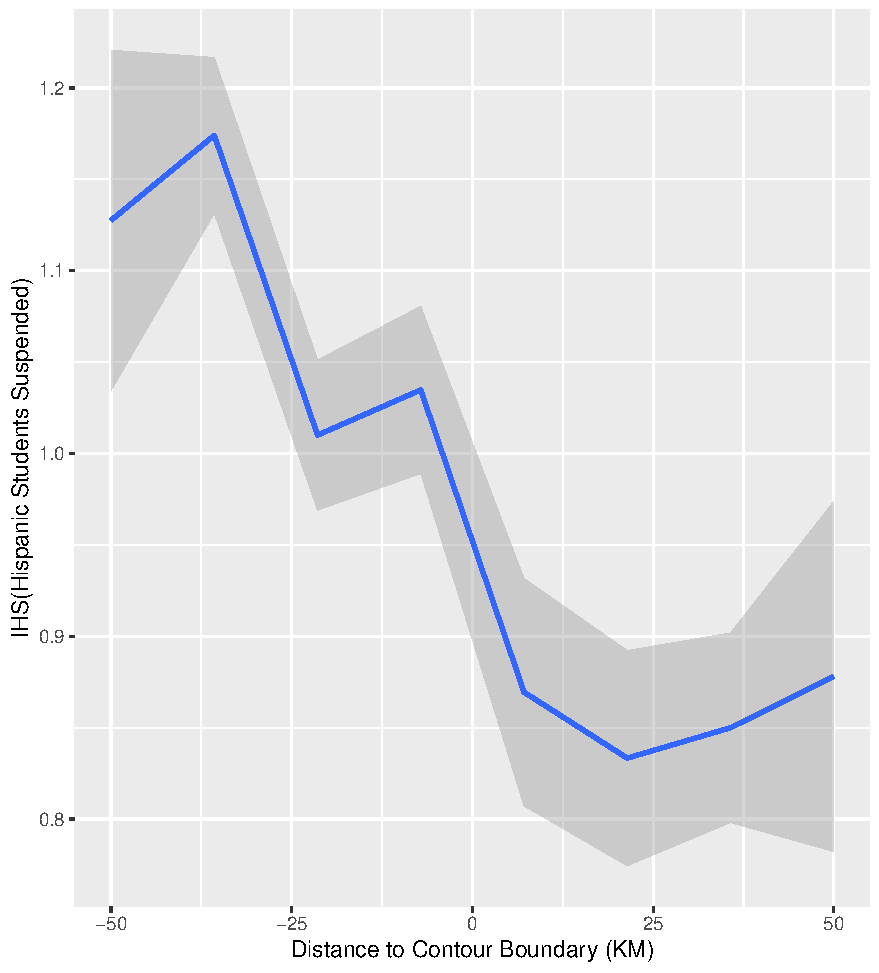
\includegraphics[width=12cm]{../../analysis/Output/graphs/hispanicsuspensions.pdf}
%
%\textit{Notes:} The figure presents data at a school level, where a smoothed average of the inverse hyperbolic sine transformed counts of Hispanic students suspended is plotted against the distance of the school to the closest Spanish Language Television station contour boundary. Positive distances denote schools that are located within the boundary, while negative distances denote schools outside of them.
%\end{figure} 



\begin{figure}[!hbtp]
\centering
\caption{Coverage map for TV station WUVC-DT}\label{f:contour_example}
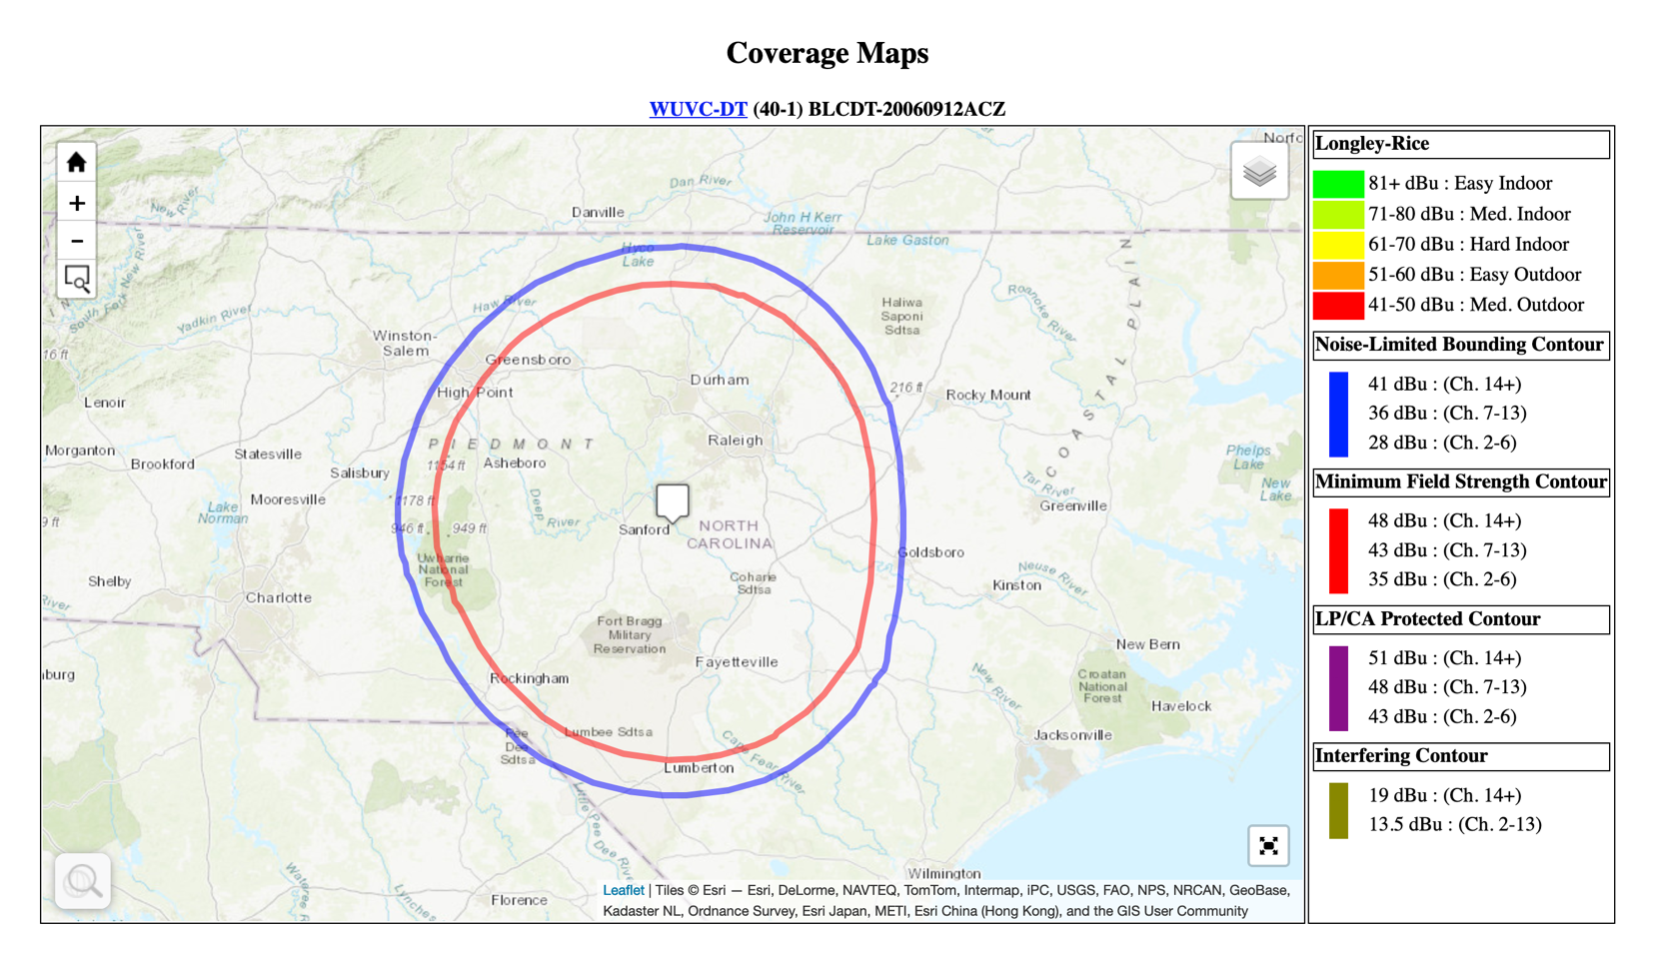
\includegraphics[width=14.4cm]{../../analysis/Output/img/ContourExample.png}
\end{figure} 

\begin{figure}[!hbtp]
\centering
\caption{Map of coverage contours of Spanish Language TV stations and public schools in the US}\label{f:contours_schools}
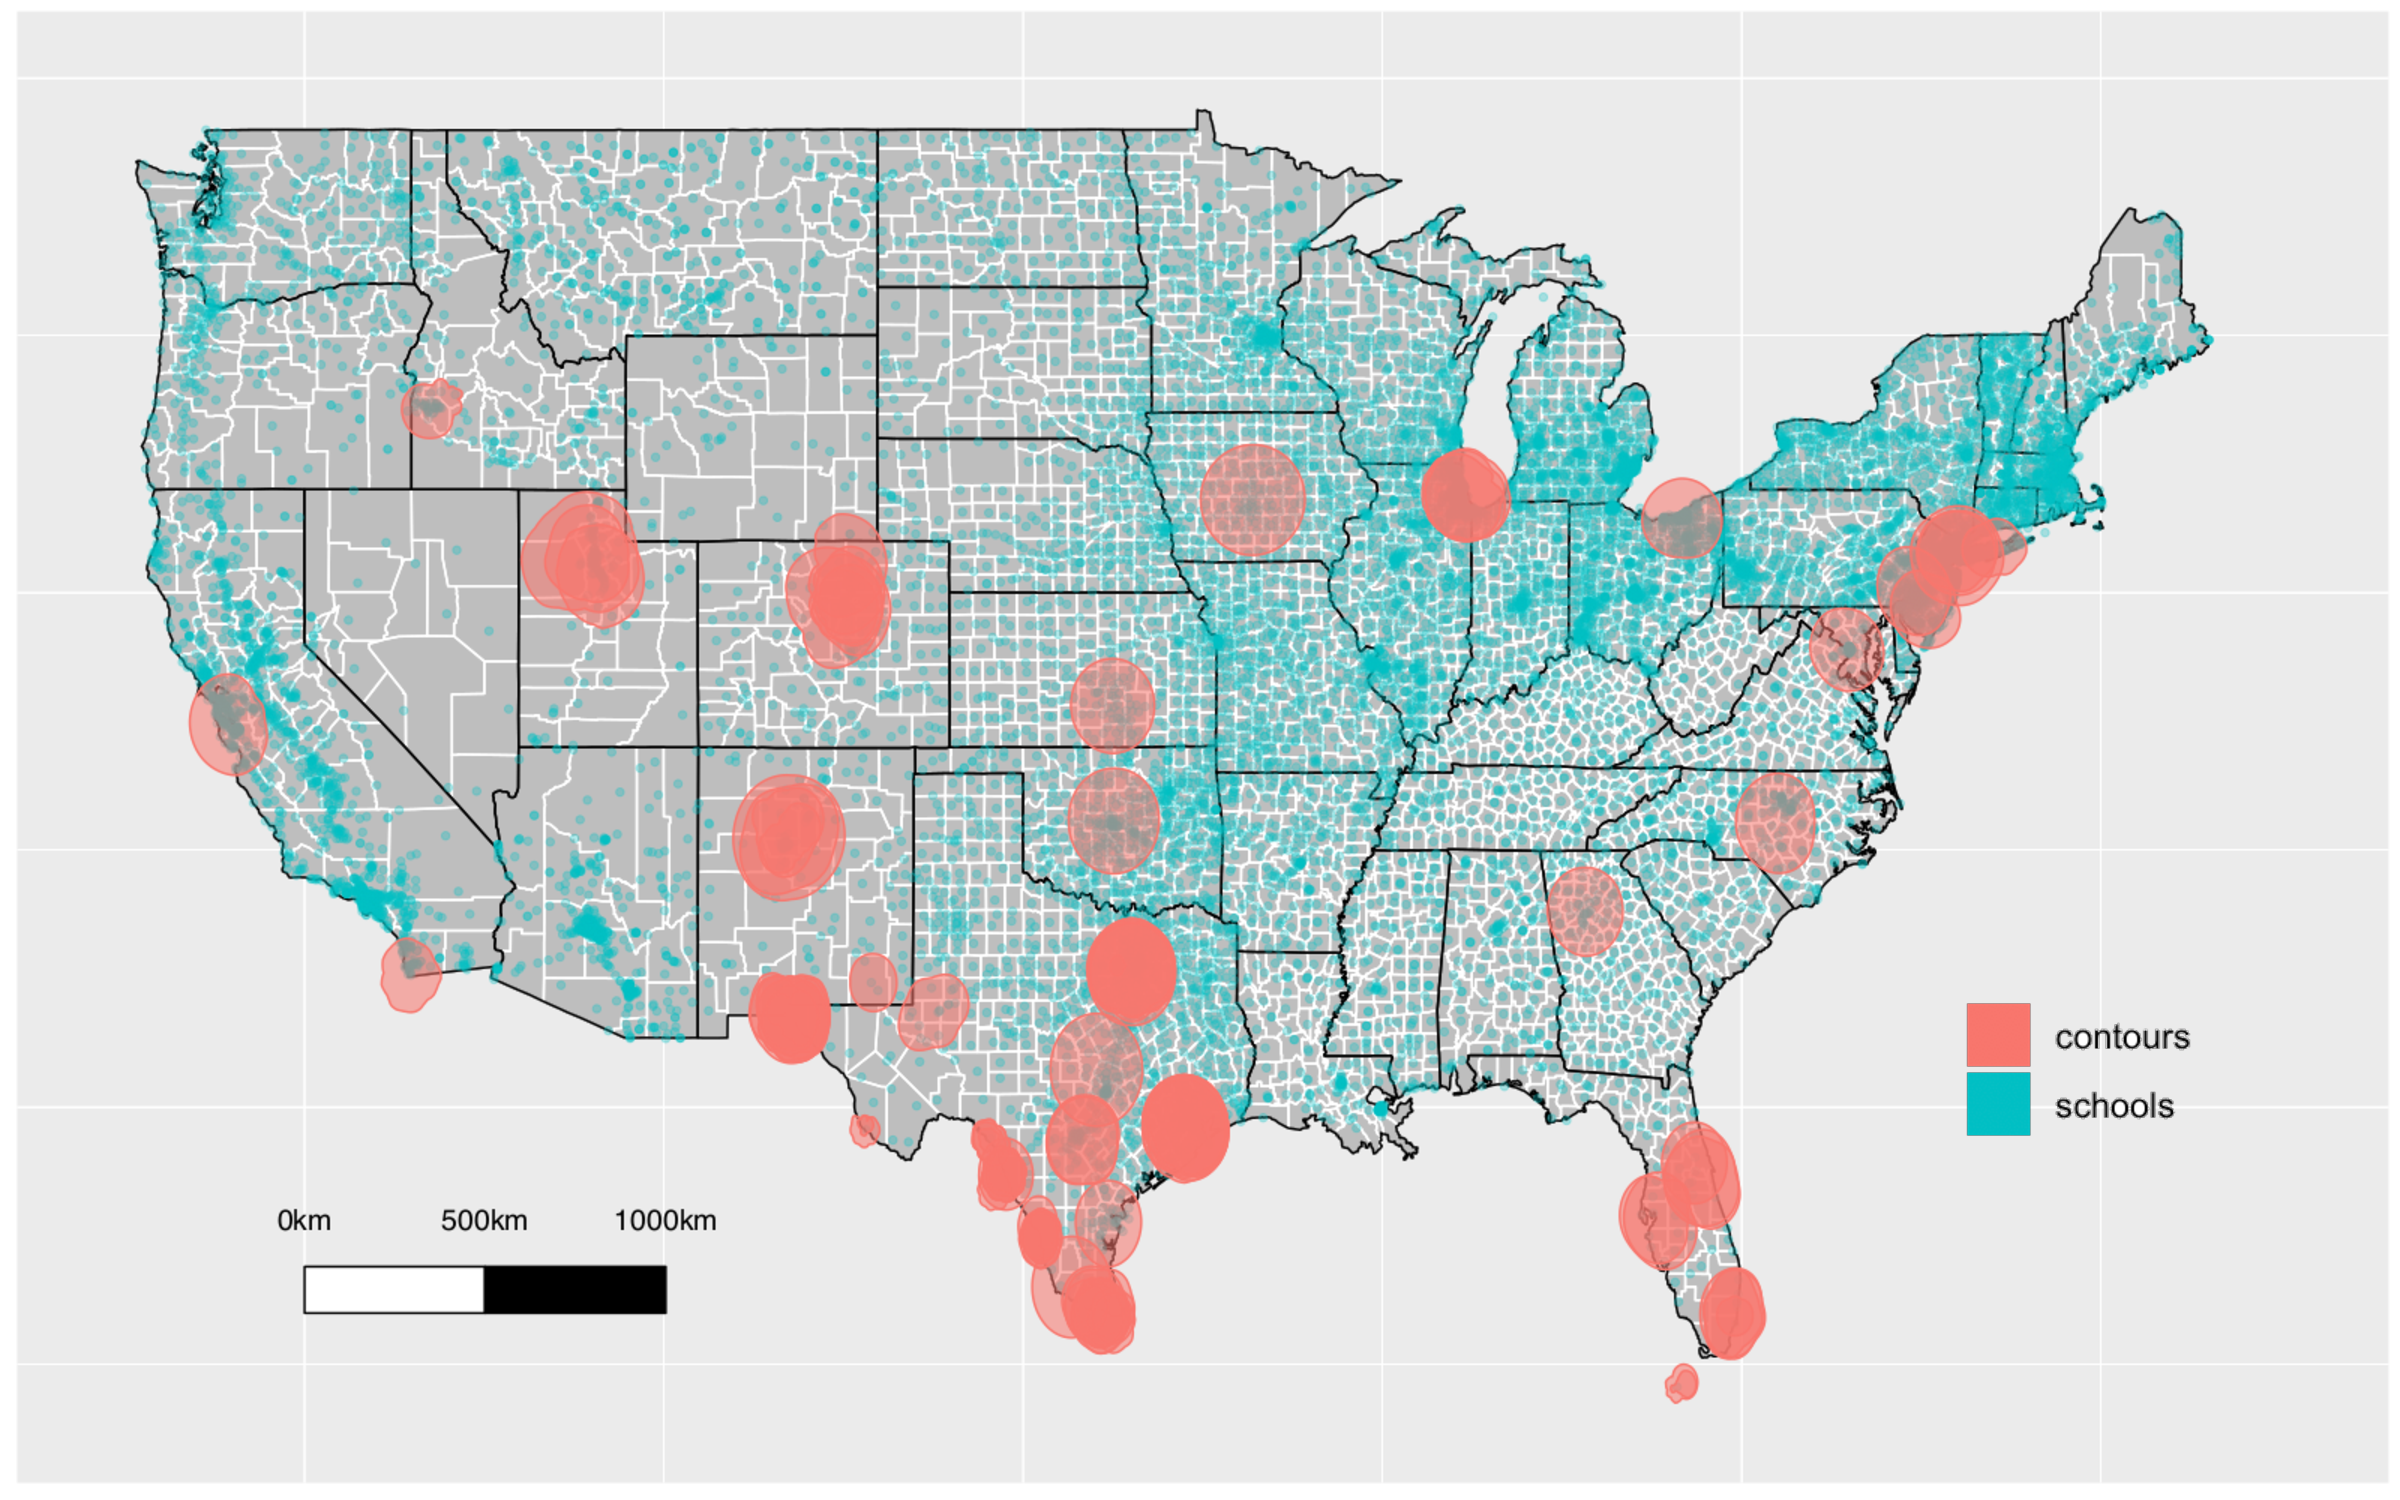
\includegraphics[width=14.4cm]{../../analysis/Output/img/Schools_pretty2.pdf}
\end{figure} 

\begin{figure}[!hbtp]
\centering
\caption{Minutes of TV watched across the coverage contour}\label{f:atus}
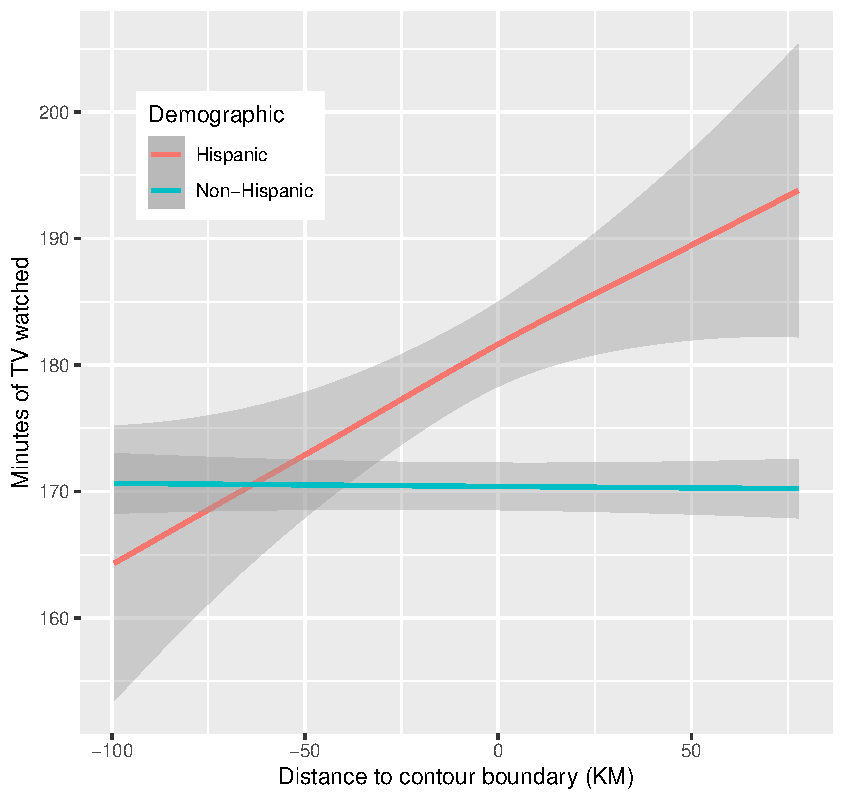
\includegraphics[width=14.5cm]{../../analysis/Output/graphs/atus.pdf}
\caption*{Lowess smoothed minutes of television watched by distance to SLTV coverage contour boundary. Negative values indicate individuals outside of a contour (no SLTV). Minutes of TV watched are residualized by individual level age, age$^2$, sex, and county level controls for log(income), log(population) and percent Hispanic. }
\end{figure} 


\clearpage

%\subsection{Tables}
%
%Table plan:
%\begin{enumerate}
%\item $<X>$ Summary stats table: ATUS data, education (school level), transcript data, Safegraph data
%\item $<X>$ ATUS: first stage (93), children (99), ATUS: parents (97),
%\item $<X>$ Education: top performance: gifted, SAT/ACT, AP passed, 
%\item $<X> $Education: identity
%\item $<X>$ Transcript: identity
%\item $<X>$ Safegraph: identity
%\end{enumerate}
%
%Appendix:
%\begin{enumerate}
%\item Migration table
%\item $<X>$ foreign born (94)
%\item Education: robustness
%\item Education: robustness spatial (SAR lag, SAR error)
%\item $<X>$ Education: more top performance
%\item Education: bottom performance?
%\item Transcript: bad identity
%\item Additional robustness
%\end{enumerate}

\expandableinput{../../analysis/Output/regs/summary_main.tex}
\expandableinput{../../analysis/Output/regs/atus_main.tex}
\expandableinput{../../analysis/Output/regs/edu_main.tex}
\expandableinput{../../analysis/Output/regs/edu_mech.tex}
\expandableinput{../../analysis/Output/regs/transcript_main.tex}
\expandableinput{../../analysis/Output/regs/safegraph_main.tex}


%%%%%%%%%%%%%%%%%%%%%%
%%%%%%%%%%%%%%%%%%%%%%

%ONLINE APPENDIX MATERIAL


\clearpage

\singlespacing

\setcounter{footnote}{0}

\setcounter{section}{0}

\setcounter{page}{1}
\renewcommand\thepage{A.\arabic{page}}

\renewcommand*{\theHsection}{\arabic{section}.\arabic{section}} 

\renewcommand*{\theHfigure}{\arabic{section}.\arabic{figure}} 
\setcounter{figure}{0}
\renewcommand\thefigure{A.\arabic{figure}}


\renewcommand*{\theHtable}{\arabic{section}.\arabic{table}} 
\setcounter{table}{0}
\renewcommand\thetable{A.\arabic{table}}

\renewcommand{\thesection}{Appendix \Alph{section}}



\begin{center}
\Large ONLINE APPENDIX
\end{center}

\section{Auxiliary data sources} \label{a:auxiliarydata}

In addition to the primary data sources described in Section~\ref{s:data}, we also use a number of auxiliary data sources for the empirical analysis.


\paragraph{Migration data}

Data on migration comes from the 2011-2015 American Community Survey (ACS), which reports the number of people moving from each origin county to destination county (aggregated over the four years).\footnote{ Historically, approximately 15\% of the ACS migration data has been allocated, or imputed based on salient characteristics (United States Census Bureau \cite{noauthor_american_2020}). } This sample also contains migration flows by Hispanic origin, allowing us to determine whether they move based on geographic boundaries.

The migration data from the ACS is provided at the origin county-destination county level. Given the relative size of a county, to define whether a county is inside a coverage contour or not, we further impose that at least 95\% of the area that the county encompasses must be inside of the coverage contour.\footnote{ Results are robust to different area cut-offs for a county to be considered inside the coverage contour.} 


\paragraph{American Time Use (ATUS)}

\paragraph{Civil Rights Data Collection (CRDC)}

The outcome data from the CRDC can be split into two categories:
\begin{itemize}
\item \textbf{Academic Achievements:} We focus on two outcomes that track the effect of television on the top end of the academic distribution of students: the number of Advanced Placement (AP) classes students enrol in and pass, as well as the number of students placed into gifted programs, and one outcome on the bottom: the number of students with Limited English Proficiency (LEP).

The AP program is administered by the College Board, and defines a standardized college-level curriculum that is taught to high school students in AP Classes. In conjunction with AP Classes, AP Exams are national examinations which are designed to test mastery of material taught in AP classes. These exams are scored on a scale ranging from 1 to 5, with scores below a 3 marked as a failed exam. Even among the students who select into these classes (22\% in 2015\footnote{ Data computed from number of high school graduates in 2015 (National Student Clearinghouse Research Center,\cite{noauthor_high_2015}), and number of seniors who sat an AP exam in 2015. This is how the College Board currently tracks national AP participation (no comparable summary statistic was released in 2015) (College Board,\cite{noauthor_ap_2015})}), a substantial number of students who take these exams fail them - approximately 35\% (College Board\cite{noauthor_ap_2020}). 

Gifted and talented programs are ``programs during regular school hours that provide special educational opportunities including accelerated promotion through grades and classes and an enriched curriculum for students who are endowed with a high degree of mental ability or who demonstrate unusual physical coordination, creativity, interest, or talent." (CRDC\cite{noauthor_master_2016}) These programs, while not mandatory, are common across school districts, and vary in their implementation. % HOW MANY STUDENTS?

LEP students (also called English Learner students) are students that, as a result of their limited command over the English language, have difficulty participating in regular school activities.\footnote{The specific definition of a LEP student depends on individual state regulation, but must also satisfy the criteria outlined under Title IX of the Elementary and Secondary Education Act (US Department of Education,\cite{noauthor_elementary_2004}). The most salient features of Title IX are that students must either not speak English as a native language or come from an environment where non-English languages are dominant, and also face substantial difficulty in engaging with others on the basis of their English ability.} 9\% of all public school students are considered LEP, and while students are placed into the program is at the discretion of individual school districts, all districts must provide language assistance services and have staff qualified to implement the LEP programs.\footnote{ Department of Justice and Department of Education,\cite{noauthor_ensuring_2015} contains a full enumeration of the responsibilities school districts have. It further includes requirements such as ensuring equal access to various school programs etc. } 

\item \textbf{Disciplinary Issues:} Three forms of academic discipline are considered as outcome variables: the number of out of school suspensions, the number of absences, and the amount of harassment and bullying on the basis of race/ethnicity experienced by students.

Out of school suspensions are instances ``in which a child is temporarily removed from his/her regular school for at least half a day (but less than the remainder of the school year) for disciplinary purposes to another setting (e.g., home, behavior center)." (CRDC,\cite{noauthor_master_2016}) We consider only students without disabilities, and note that depending on school policy, educational services may still be provided during this time.\footnote{Students with disabilities served under IDEA face substantially different suspension policy.}

A chronically absent student is one ``who is absent 15 or more school days during the school year. A student is absent if he or she is not physically on school grounds and is not participating in instruction or instruction-related activities at an approved off-grounds location for at least half the school day." (CRDC,\cite{noauthor_master_2016}) Each day for which a student is absent for 50 percent or more of the school day is counted. Absences are counted regardless of whether they are excused or not, and so include absences due to illness, needing to care for a family member, or simple truancy.

Harassment or bullying on the basis of race, color, or national origin ``refers to intimidation or abusive behavior toward a student based on actual or perceived race, color, or national origin. Harassing conduct may take many forms, including verbal acts and name-calling, as well as non-verbal behavior, such as graphic and written statements, or conduct that is physically threatening, harmful or humiliating. The conduct can be carried out by school employees, other students, and non-employee third parties. Bullying on the basis of race, color, or national origin constitutes racial harassment." (CRDC,\cite{noauthor_master_2016}) Though there are other categories of bullying and harassment reported (and other types of infractions and disciplinary measures taken), these are less directly relevant to the question at hand.


\end{itemize}

Notably, all the outcome information described above is also provided for Hispanic subpopulations --- hence, the outcome of interest is generally the number of Hispanic students passing AP tests, or being bullied on the basis of their ethnicity, etc. These variables are all reported at the school level. 
dummies for whether the school contains a primary school, middle school, and high school. 


% sample problems
% \footnote{ In practice, this data is not released to the public every year. Furthermore, not all schools report all data (or correct data) required of them, which is why the number of observations for different variables in this dataset fluctuates. Some data, such as that on AP examinations, are not mandatory, but the bulk of outcome variables are, with non-compliance on the mandatory data typically representing $<1\%$ of total data.} 

Controls at the county level are sourced from IPUMS and consist of basic relevant demographic information: population, income, percent of county that is Hispanic etc. County level data is mapped to its relevant location using census data as well. 

% TODO: propagate errors based on the margin of error

Finally, data attached to specific outcomes are discussed under their relevant section.


\paragraph{archive.org transcript data} 
Appendix Table~\ref{t:transcript_keywords} Panel A contains the list of word stubs for Hispanic countries. Panel B contains a list of common words relating to education. Panel C contains a list of telenovelas with good role models that aired before 2015.

though noisy, aggregating at the parent network level is XX given that more than half the content in SLTV stations are either sourced internationally or produced for national consumption

\paragraph{Safegraph foot-traffic data}
% on names
Unlike the names of firm principals, there is no readily available or standardized method to determine whether a firm's name is a `Hispanic name' or not. Although a machine learning approach is still theoretically possible under these circumstances, a quick visual inspection of the data revealed that a relatively low percentage of firms had names that were explicit tied to a Hispanic identity---hence, many approaches would likely identify a significant number of false positives.

In order to be conservative and ensure that firms identified as bearing Hispanic names actually are such, we construct a measure that classifies a firm name as Hispanic if it contains certain keywords that are explicitly associated with a Hispanic identity. These keywords are split into three major categories: (1) References to countries in Latin America or Latin America itself. Firms that include the base forms of country names in Latin America are considered to be explicitly referencing a Hispanic identity (examples include: `Cuban Guys 102, LLC' , `Bravo Latino Brands, LLC.') (2) Names containing common one of the top 50 most Spanish words that are not also present in English (examples include: `La Joya Estates, Ltd.', `Conselho Nacional De Saude Mental E Medicina Psicossomatica Inc.'), and (3) Names containing common Hispanic foods. (examples include: `Charlie Cactus Tacos, LLC', `Taqueria Casas 2 Inc.') Due to the lack of a systemic means to construct this last category, I conduct robustness checks dropping this category; results do not substantially change when omitting this third category. Table \ref{firm_class} contains a list of these keywords as well as some additional detail on the classification process.

Out of our sample, 1.1\% of firms meet this criteria (1\% if omitting the food-based names). A manual check of firms that are classified as Hispanic also confirms that the firm name classification process succeeds.



\paragraph{Geocoding}

Geocoding by ArcGIS is successful over 99.9\% of the time. Schools not successfully geocoded are dropped from the sample.

Distance for counties are computed by minimum distances




\clearpage

\section{Additional figures and tables}

% TODO: map contours by parent network?
% TODO: map all POIs

\begin{table}[!h]
	\centering
	\captionsetup{skip=1.5pt}
	\caption{Influence of Spanish Language Television on Migration Between Counties - Origin Sample} \label{t:mig_orig}
	\scalebox{.7}{
		\begin{threeparttable}
			\begin{tabular}{lcccccccccc}
				\hline\hline\addlinespace
				& \multicolumn{3}{c}{IHS(\# Hispanic Migrants)} \\
				\cline{2-4} 
				Panel A: Origin County Inside Contour&  (1) & (2) & (3) \\
                                \hline\addlinespace
Dummy: Destination Outside TV Contour & $-$0.387$^{***}$ & $-$0.286$^{***}$ & $-$0.280$^{***}$ \\ 
  & (0.048) & (0.044) & (0.044) \\ 
 TV Dummy $\times$ Distance to Origin & $-$0.003$^{**}$ & $-$0.004$^{***}$ & $-$0.004$^{***}$ \\ 
  & (0.001) & (0.001) & (0.001) \\ 
 TV Dummy $\times$ Distance to Destination & 0.001 & $-$0.002$^{*}$ & $-$0.002 \\ 
  & (0.001) & (0.001) & (0.001) \\ 
 Distance from Contour to Origin (KM) & 0.001 & 0.003$^{*}$ & 0.003 \\ 
  & (0.002) & (0.002) & (0.002) \\ 
 Distance from Contour to Destination (KM) & $-$0.001 & 0.002 & 0.002 \\ 
  & (0.001) & (0.001) & (0.001) \\ 
 Origin Log(Population) & 0.146$^{***}$ & 0.161$^{***}$ & 0.150$^{***}$ \\ 
  & (0.020) & (0.017) & (0.021) \\ 
 Destination Log(Population) & 0.150$^{***}$ & 0.136$^{***}$ & 0.125$^{***}$ \\ 
  & (0.014) & (0.013) & (0.016) \\ 
 Origin \% Hispanic &  & 0.792$^{***}$ & 0.881$^{***}$ \\ 
  &  & (0.103) & (0.141) \\ 
 Destination \% Hispanic &  & 1.485$^{***}$ & 1.573$^{***}$ \\ 
  &  & (0.122) & (0.141) \\ 
 Origin Log(Income) &  &  & 0.093 \\ 
  &  &  & (0.094) \\ 
 Destination Log(Income) &  &  & 0.090 \\ 
  &  &  & (0.078) \\ 
Observations & 8,479 & 8,479 & 8,479 \\ 
\hline\addlinespace
Panel B: Origin County Outside Contour & & & \\ 
\hline\addlinespace
 Dummy: Destination Inside TV Contour & $-$0.078 & $-$0.123 & $-$0.120 \\ 
  & (0.108) & (0.096) & (0.096) \\ 
 TV Dummy $\times$ Distance to Origin & $-$0.003$^{*}$ & $-$0.004$^{***}$ & $-$0.004$^{***}$ \\ 
  & (0.002) & (0.001) & (0.001) \\ 
 TV Dummy $\times$ Distance to Destination & $-$0.004$^{***}$ & $-$0.002 & $-$0.002 \\ 
  & (0.001) & (0.001) & (0.001) \\ 
 Distance from Contour to Origin (KM) & $-$0.0003 & 0.001 & 0.001 \\ 
  & (0.001) & (0.001) & (0.001) \\ 
 Distance from Contour to Destination (KM) & $-$0.001$^{***}$ & $-$0.001$^{***}$ & $-$0.001$^{***}$ \\ 
  & (0.0002) & (0.0003) & (0.0003) \\ 
 Origin Log(Population) & 0.164$^{***}$ & 0.131$^{***}$ & 0.094$^{***}$ \\ 
  & (0.017) & (0.021) & (0.026) \\ 
 Destination Log(Population) & 0.150$^{***}$ & 0.128$^{***}$ & 0.125$^{***}$ \\ 
  & (0.023) & (0.020) & (0.021) \\ 
 Origin \% Hispanic &  & 1.328$^{***}$ & 1.611$^{***}$ \\ 
  &  & (0.295) & (0.329) \\ 
 Destination \% Hispanic &  & 1.485$^{***}$ & 1.481$^{***}$ \\ 
  &  & (0.293) & (0.318) \\ 
 Origin Log(Income) &  &  & 0.407$^{**}$ \\ 
  &  &  & (0.193) \\ 
 Destination Log(Income) &  &  & 0.003 \\ 
  &  &  & (0.087) \\ 
Observations & 4,062 & 4,062 & 4,062 \\         
\hline\addlinespace
                                Origin F.E. & Yes & Yes  & Yes\\
				\addlinespace\hline\hline
			\end{tabular}
			\begin{tablenotes}[flushleft]
				\item \textit{Notes:} The table presents coefficient estimates from regressions at the county-county level, only keeping origin counties within 100 KM of a contour boundary. The dependent variables are inverse hyperbolic sine transformed counts of Hispanic migrants from the origin county to the destination county. The key dependent variable of interest is the TV Dummy, which tracks whether the destination county is inside or outside the TV contour. This is interacted with the distance to the boundary for both the origin and destination county. County controls include log income, log population, and percentage county Hispanic for both origin and destination county. All regressions also contain origin county fixed effects. Standard errors are given in parentheses. *, **, and *** denote statistical significance at the 10\%, 5\%, and 1\% levels, respectively.
			\end{tablenotes}
		\end{threeparttable}
	}
\end{table}
\begin{table}[!h]
	\centering
	\captionsetup{skip=1.5pt}
	\caption{Influence of Spanish Language Television on Migration Between Counties - Destination Sample} \label{mig_dest}
	\scalebox{.7}{
		\begin{threeparttable}
			\begin{tabular}{lcccccccccc}
				\hline\hline\addlinespace
				& \multicolumn{3}{c}{IHS(\# Hispanic Migrants)} \\
				\cline{2-4} 
				Panel A: Destination County Inside Contour&  (1) & (2) & (3) \\
                                \hline\addlinespace
 Dummy: Origin Outside TV Contour & $-$0.410$^{***}$ & $-$0.356$^{***}$ & $-$0.349$^{***}$ \\ 
  & (0.088) & (0.082) & (0.081) \\ 
 TV Dummy $\times$ Distance to Destination & $-$0.007$^{***}$ & $-$0.008$^{***}$ & $-$0.008$^{***}$ \\ 
  & (0.003) & (0.003) & (0.003) \\ 
 TV Dummy $\times$ Distance to Origin & $-$0.002 & $-$0.004$^{**}$ & $-$0.004$^{*}$ \\ 
  & (0.002) & (0.002) & (0.002) \\ 
 Distance from Contor to Destination (KM) & 0.002 & 0.004$^{**}$ & 0.004$^{**}$ \\ 
  & (0.002) & (0.002) & (0.002) \\ 
 Distance from Contour to Origin (KM) & 0.001 & 0.004 & 0.003 \\ 
  & (0.002) & (0.002) & (0.002) \\ 
 Destination Log(Population) & 0.179$^{***}$ & 0.181$^{***}$ & 0.175$^{***}$ \\ 
  & (0.019) & (0.016) & (0.019) \\ 
 Origin Log(Population) & 0.115$^{***}$ & 0.117$^{***}$ & 0.102$^{***}$ \\ 
  & (0.018) & (0.017) & (0.020) \\ 
 Destination \% Hispanic &  & 1.384$^{***}$ & 1.428$^{***}$ \\ 
  &  & (0.183) & (0.205) \\ 
 Origin \% Hispanic &  & 0.813$^{***}$ & 0.949$^{***}$ \\ 
  &  & (0.182) & (0.203) \\ 
 Destination Log(Income) &  &  & 0.041 \\ 
  &  &  & (0.099) \\ 
 Origin Log(Income) &  &  & 0.138 \\ 
  &  &  & (0.109) \\ 
Observations & 4,338 & 4,338 & 4,338 \\ 
\hline\addlinespace
Panel B: Origin County Outside Contour & & & \\ 
\hline\addlinespace
 Dummy: Origin Inside TV Contour & $-$0.140 & $-$0.194 & $-$0.193 \\ 
  & (0.152) & (0.144) & (0.144) \\ 
 TV Dummy $\times$ Distance to Destination & $-$0.004$^{*}$ & $-$0.007$^{***}$ & $-$0.007$^{***}$ \\ 
  & (0.002) & (0.002) & (0.002) \\ 
 TV Dummy $\times$ Distance to Origin & $-$0.007$^{**}$ & $-$0.004 & $-$0.004 \\ 
  & (0.003) & (0.003) & (0.003) \\ 
 Distance from Contor to Destination (KM) & $-$0.0003 & 0.002 & 0.002 \\ 
  & (0.002) & (0.001) & (0.001) \\ 
 Distance from Contour to Origin (KM) & $-$0.001$^{***}$ & $-$0.002$^{***}$ & $-$0.002$^{***}$ \\ 
  & (0.0004) & (0.0004) & (0.0004) \\ 
 Destination Log(Population) & 0.253$^{***}$ & 0.169$^{***}$ & 0.153$^{***}$ \\ 
  & (0.041) & (0.023) & (0.030) \\ 
 Origin Log(Population) & 0.182$^{***}$ & 0.181$^{***}$ & 0.181$^{***}$ \\ 
  & (0.035) & (0.030) & (0.034) \\ 
 Destination \% Hispanic &  & 2.324$^{***}$ & 2.471$^{***}$ \\ 
  &  & (0.389) & (0.411) \\ 
 Origin \% Hispanic &  & 1.276$^{**}$ & 1.253$^{**}$ \\ 
  &  & (0.602) & (0.584) \\ 
 Destination Log(Income) &  &  & 0.181 \\ 
  &  &  & (0.196) \\ 
 Origin Log(Income) &  &  & $-$0.015 \\ 
  &  &  & (0.192) \\ 
Observations & 1,659 & 1,659 & 1,659 \\        
\hline\addlinespace
                                Destination F.E. & Yes & Yes  & Yes\\
				\addlinespace\hline\hline
			\end{tabular}
			\begin{tablenotes}[flushleft]
				\item \textit{Notes:} The table presents coefficient estimates from regressions at the county-county level, only keeping destination counties within 100 KM of a contour boundary. The dependent variables are inverse hyperbolic sine transformed counts of Hispanic migrants from the origin county to the destination county. The key dependent variable of interest is the TV Dummy, which tracks whether the destination county is inside or outside the TV contour. This is interacted with the distance to the boundary for both the origin and destination county. County controls include log income, log population, and percentage county Hispanic for both origin and destination county. All regressions also contain destination county fixed effects. Standard errors are given in parentheses. *, **, and *** denote statistical significance at the 10\%, 5\%, and 1\% levels, respectively.
			\end{tablenotes}
		\end{threeparttable}
	}
\end{table}

\expandableinput{../../analysis/Output/regs/atus_foreign.tex}

\expandableinput{../../analysis/Output/regs/edu_magnitude.tex}
\expandableinput{../../analysis/Output/regs/edu_abs.tex}
\expandableinput{../../analysis/Output/regs/edu_extra_achieve.tex}
\clearpage
\expandableinput{../../analysis/Output/regs/edu_robust.tex}
\clearpage
\expandableinput{../../analysis/Output/regs/edu_retain.tex}

\expandableinput{../../analysis/Output/regs/edu_mech_placebo.tex}
\expandableinput{../../analysis/Output/regs/edu_mech_abs.tex}

\expandableinput{../../analysis/Output/regs/transcript_abs.tex}
\expandableinput{../../analysis/Output/regs/atus_edu.tex}

\expandableinput{../../analysis/Output/regs/safegraph_abs.tex}


%\begin{table}[!h]
	\centering
	\captionsetup{skip=1.5pt}
	\caption{Robustness of Influence of Spanish Language Television on Hispanic Students Passing the AP} \label{edu_ap_robust}
	\scalebox{.8}{
		\begin{threeparttable}
			\begin{tabular}{lcccccccccc}
				\hline\hline\addlinespace
				 & \multicolumn{6}{c}{\textit{IHS(\# Hispanic Students Passing AP)}}\\
				&  (1) & (2) & (3) & (4) & (5) & (6) \\
                                \hline\addlinespace
 TV Dummy & 0.039$^{***}$ & 0.049$^{***}$ & 0.044$^{***}$ & 0.044$^{***}$ & 0.036$^{***}$ & 0.032$^{*}$ \\ 
  & (0.013) & (0.017) & (0.016) & (0.017) & (0.013) & (0.018) \\ 
 TV Dummy $\times$ Distance to Boundary & 0.0003 & 0.0001 & 0.001 & 0.001$^{*}$ & 0.0001 & 0.001 \\ 
  & (0.0002) & (0.001) & (0.001) & (0.0004) & (0.0004) & (0.001) \\ 
 Distance to Boundary (meters) & 0.001 & 0.012$^{***}$ & 0.006$^{***}$ & 0.006$^{***}$ & 0.003$^{**}$ & 0.001 \\ 
  & (0.001) & (0.003) & (0.002) & (0.002) & (0.002) & (0.004) \\ 
 \# Hispanic Students & 0.001$^{***}$ & 0.001$^{***}$ & 0.001$^{***}$ & 0.001$^{***}$ & 0.001$^{***}$ & 0.001$^{***}$ \\ 
  & (0.00004) & (0.00004) & (0.00005) & (0.0002) & (0.00004) & (0.0001) \\ 
 Total APs Passed &  &  &  &  & 0.003$^{***}$ &  \\ 
  &  &  &  &  & (0.0001) &  \\ 
Observations & 2,205 & 2,205 & 1,525 & 1,525 & 1,525 & 1,095 \\ 
\hline\hline\addlinespace
                                County/School Controls & Yes & Yes  & Yes & Yes & Yes & Yes\\
                                Distance Cutoff (KM) & 100 & 100 & 50 & 50 & 50 & 33 $\frac{1}{3}$ \\
                                Distance$^{2}$ Interaction & No & Yes & No & No & No & No \\
                                County F.E. & No & No & No & Yes & No & No  \\
				\addlinespace\hline\hline
			\end{tabular}
			\begin{tablenotes}[flushleft]
				\item \textit{Notes:} The table presents coefficient estimates from regressions at the school level. The dependent variable is the inverse hyperbolic sine transformed counts of Hispanic students who have passed an AP exam. The key dependent variable of interest is the TV Dummy, which tracks whether the school is within a coverage contour boundary for a Spanish language television station. This is interacted with the distance to the boundary. County and school controls include log income, log population, percentage county Hispanic for the county which the school is located in, and the number of teachers, total number of students at the school, and dummies for whether the school contains a primary, middle, and high school division. Various distance cut-offs to the boundary are presented, as well as the TV dummy interacted with the square of the distance. All regressions also control for the number of Hispanic students enrolled at the school. Standard errors are given in parentheses. *, **, and *** denote statistical significance at the 10\%, 5\%, and 1\% levels, respectively.
			\end{tablenotes}
		\end{threeparttable}
	}
\end{table}
%\begin{table}[!h]
	\centering
	\captionsetup{skip=1.5pt}
	\caption{Spatial Robustness of Influence of Spanish Language Television on Hispanic Victims of Ethnicity-Based Harassment} \label{edu_spatial}
	\scalebox{.8}{
		\begin{threeparttable}
			\begin{tabular}{lcccccccccc}
				\hline\hline\addlinespace
				 & \multicolumn{3}{c}{\textit{IHS(\# Hispanic Victims of Harassment)}}\\
				&  (1) & (2) & (3) \\
                                \hline\addlinespace
 TV Dummy & 0.003$^{**}$ & 0.002$^{***}$ & 0.003$^{*}$ \\ 
  & (0.001) & (0.001) & (0.002) \\ 
 TV Dummy $\times$ Distance to Boundary & $-$0.0001$^{**}$ & $-$0.0001$^{***}$ & $-$0.0001$^{**}$ \\ 
  & (0.00002) & (0.00001) & (0.00003) \\ 
\hline\hline\addlinespace
Observations & 40,811 & 40,811 & 40,811 \\ 
Log Likelihood &  & $-$4,304.916 & $-$4,299.820 \\ 
$\sigma^{2}$ &  & 0.072 & 0.072 \\ 
Akaike Inf. Crit. &  & 8,629.833 & 8,619.640 \\ 
Wald Test (df = 1) &  & 686.149$^{***}$ & 686.981$^{***}$ \\ 
LR Test (df = 1) &  & 657.312$^{***}$ & 667.505$^{***}$ \\ 
\hline \addlinespace
                                County/School Controls & Yes & Yes  & Yes \\
                                Model & OLS & SAR Lag & SAR Error \\
				\addlinespace\hline\hline
			\end{tabular}
			\begin{tablenotes}[flushleft]
				\item \textit{Notes:} The table presents coefficient estimates from regressions at the school level, only keeping schools within 100 KM of a contour boundary. The dependent variable is the inverse hyperbolic sine transformed counts of Hispanic students who are bullied or harassed on the basis of their ethnicity. The key dependent variable of interest is the TV Dummy, which tracks whether the school is within a coverage contour boundary for a Spanish language television station. This is interacted with the distance to the boundary. County and school controls include log income, log population, percentage county Hispanic for the county which the school is located in, and the number of teachers, total number of students at the school, and dummies for whether the school contains a primary, middle, and high school division. The SAR Lag model is a spatial autoregressive lag model and the SAR Error model is a spatial autoregressive error model, both with weight matrices based on 4 nearest neighbours. Standard errors are given in parentheses. *, **, and *** denote statistical significance at the 10\%, 5\%, and 1\% levels, respectively.
			\end{tablenotes}
		\end{threeparttable}
	}
\end{table}




\begin{table}[!h]
	\centering
	\captionsetup{skip=1.5pt}
	\caption{TV transcript keywords} \label{t:transcript_keywords}
	\scalebox{.8}{
	 	\begin{threeparttable}
			\begin{tabular}{llcccccccc}
				\hline\hline\addlinespace
    \textit{Panel A: Hispanic references} & mexic, bolivia, chile, argentin, venezuela, beliz, costa rica, salvador, guatemala \\
&  hondur, nicaragua, panama, colombia, ecuador, guyana, paragua, peru \\
& urugu, cuba, dominican, puerto, latin \\
				\addlinespace\hline
\textit{Panel B: Education references} &educación , enseñanza, colegio, escuela, universidad, estudio, estudiar, estudiante\\  
& alumna, alumno, profesora, profesor, maestro, maestra, clase, rango, grado \\
& aprender, mates, matematicas \\
\hline
\textit{Panel C: Role model references} & Vivan los niños, Alegrijes y rebujos, Aventuras en El tiempo, amigos por siempre \\
					& Misión S.O.S., Carrusel y El abuelo y Yo, El Juego de la Vida, De pocas pulgas\\
					& luz Clarita, Serafín, 31 minutos, Bizbirije, Odisea Burbujas, El Tesoro del Saber \\
					& Topo Gigio, Once Niñas y Niños \\		 		
				\addlinespace\hline\hline
			\end{tabular}
			\begin{tablenotes}[flushleft]
				\item \textit{Notes:} Television transcripts are classified as containing a reference name if any keyword (or program title in Panel C) in the panel is exactly matched within the word, ignoring case. Panel A contains the list of word stubs for Hispanic countries. Panel B contains a list of common words relating to education. Panel C contains a list of telenovelas with good role models for children that aired before 2015.
			\end{tablenotes}
		\end{threeparttable}
	}
\end{table}


\pagebreak




\end{document}


%Resources:
%https://rpubs.com/chrisbrunsdon/114718
%https://rpubs.com/corey_sparks/109650
%http://www.econ.uiuc.edu/~lab/workshop/Spatial_in_R.html
%https://rspatial.org/raster/analysis/7-spregression.html
%Conley Errors





 